\documentclass[UTF8,a4paper,autofakebold,15pt]{ctexart}

\usepackage{xeCJK}
\usepackage{fontspec}
\usepackage{ulem}
\usepackage{amsmath}
\usepackage{setspace}
\usepackage{amssymb}
\usepackage{listings}
\usepackage{titlesec}
\usepackage{multicol}
\usepackage{graphicx}
\usepackage{subfig}
\usepackage{multirow}
\usepackage[colorlinks, linkcolor=black]{hyperref}
\usepackage{geometry}
\newcommand{\ee}{\mathrm e}
\newcommand{\ii}{\mathrm i}
\usepackage{xcolor}
%\geometry{left=3cm,right=2.5cm,top=1.5cm,bottom=2.5cm}
%\setmonofont{YaHei-Consolas-Hybrid}
\lstset{
	columns=fixed, 
	tabsize=4,
	frame=none,                                          % 不显示背景边框
	numbers=left,
	backgroundcolor=\color[RGB]{245,245,244},            % 设定背景颜色
	keywordstyle=\color[RGB]{40,40,255},                 % 设定关键字颜色
	numberstyle=\footnotesize\color{darkgray},           % 设定行号格式
	commentstyle=\it\color[RGB]{0,96,96},                % 设置代码注释的格式
	basicstyle=\ttfamily,
	stringstyle=\ttfamily\slshape\color[RGB]{128,0,0},   % 设置字符串格式
	showstringspaces=false,                              % 不显示字符串中的空格
	language=verilog,                                        % 设置语言
	breaklines=true,
}

\newCJKfontfamily\sonti{STSongti-SC-Regular}[BoldFont=STSongti-SC-Bold]
%\newCJKfontfamily\heiti{SimHei}[FakeBold=3]

%\setCJKmainfont{STSongti-SC-Regular}[BoldFont=STSongti-SC-Bold]
\setCJKmonofont{STSongti-SC-Regular}[BoldFont=STSongti-SC-Bold]

\titleformat*{\section}{\centering\zihao{-2}\bfseries}

\titleformat*{\subsection}{\zihao{4}\bfseries}

\title{武汉大学计算机学院\\
	本科生课程设计报告
}
\author{}
\date{}
\setmainfont{Times New Roman}

\pagestyle{plain}
\begin{document}
	
	\begin{center}
		
	\vspace{50pt}
	{\zihao{1}\tt 武汉大学计算机学院\\\vspace{10pt}
		本科生课程设计报告}
	
	\vspace{50pt}
	
	{\heiti\zihao{2}\bf RISC-V CPU设计}
	
	\vspace{100pt}
	
	\begin{spacing}{1.5}
	\zihao{-3}
	\qquad\begin{tabular}{ll}
		专\ 业\ 名\ 称   :&计算机科学与技术(弘毅学堂)\\
		
		课\ 程\ 名\ 称   :&计算机系统综合设计\\
		
		指\ 导\ 教\ 师   :&蔡朝晖\ 副教授\\
		&陈伟清\ 高级实验师\\
		
		学\ 生\ 学\ 号   :&2020300004071\\
		
		学\ 生\ 姓\ 名   :&王骏峣
	\end{tabular}

	\end{spacing}

	\vspace{100pt}

	\zihao{3} 二〇二一年七月
	
	\end{center}
	

\newpage

	\begin{center}
	{\setmainfont{SimSun}\zihao{2}\bf 郑\ 重\ 声\ 明}
	\end{center}

	\vspace{20pt}
	
	\zihao{-3}
	本人呈交的实验报告,是在指导老师的指导下,独立进行实验工作所取得的成果,所有数据、图片资料真实可靠。尽我所知,除文中已经注明引用的内容外,本实验报告不包含他人享有著作权的内容。对本实验报告做出贡献的其他个人和集体,均已在文中以明确的方式标明。本实验报告的知识产权归属于培养单位。
	
	\vspace{20pt}
	
	本人签名:\_\_\_\_\_\_          日期:\_\_\_\_\_\_
	
\newpage

	\zihao{-2}
	
	\begin{center}
		{\bf 摘\quad 要}
	\end{center}
	
	\zihao{-4}
	
	本实验的实验目的是完成基于RISC-V架构CPU的设计,使其支持37条简单指令集,在五级流水线下能够正常处理指令、避免数据冒险和控制冒险。以及通过ISE软件将相关内容综合到SoC系统并导入FPGA开发板,并完成开发板上基于该CPU应用程序的实现。
	
	实验设计主要遵循《计算机组成与设计:硬件/软件接口 RISC-V(第五版)》\cite{ref1}中流水线架构CPU各模块的输入、输出端口,功能信号的规定以及RISC-V指令集中各个指令对应的数据周转流程与对应信号。最终设计成功与否取决仿真的波形是否与理论波形一致,以ModelSim软件仿真结果作为参考,观察在SWORD平台上的运行结果。
	
	实验内容主要包括:使用Verilog语言在提供的xgriscv文件的结构基础上修改并拓展各个模块的功能代码,使得CPU能正确执行RISC-V精简指令集:\{{\tt add, sub, and, or, lw, sw, beq, jalr, jal, ori, xor, xori, andi, addi, sll, sra, srl, slt, sltu, srai, slti, sltiu, slli, srli, lui, lb, lh, lbu, lhu, sb, sh, bne, blt, bge, bltu, bgeu, auipc}\}(注:数据在内存中以小端形式存储)。使用Venus平台编写并运行测试用的汇编代码并将其编译为机器码,在Modelsim SE 10.4环境中使用项目文件对Venus生成的机器码在设计的CPU架构上进行仿真,核对仿真产生的波形与寄存器的值和Venus平台执行结果是否相同。同时使用流水线寄存器、旁路单元、冒险控制单元等机制处理数据冒险、控制冒险。最后在 Xilinx ISE 14.7 环境中完成对总线、外设等模块的综合连线,生成SWORD设备可以读取的比特流,导入设备后测试使用情况。
	
	实验结论为:仿真产生的波形和寄存器的值与Venus执行结果相同,控制冒险与数据冒险被解决,导入SWORD开发板后可以正常运行并显示内容,证明该流水线CPU设计成功。更改综合连线后可以支持键盘、VGA等外设,说明该CPU可以支持更广泛的应用。
	
	
	{\bf 关键词:}CPU;RISC-V;流水线架构;VGA
	
\newpage

	\zihao{-2}
	
	\begin{center}
		{\bf 目\quad 录}
	\end{center}
	
	\zihao{-4}
	
	\renewcommand{\contentsname}{}
	
	\tableofcontents
	
\newpage


\section{引言}

\subsection{实验目的}

	本实验的实验目的是融会贯通计算机组成与设计课程所教授的知识,通过对知识的综合应用,加深对CPU系统各模块的工作原理及相互联系的认识。
	
	学习采用EDA(Electronic Design Automation)技术设计RISC-V单周期CPU/流水线CPU的技术与方法。
	
	培养科学研究的独立工作能力,取得CPU设计与仿真的实践和经验。
	
	了解SOC系统,并在FPGA开发板上实现简单的SOC系统。
	
	最终完成基于RISC-V架构CPU的设计,使其支持37条简单指令集,在五级流水线下能够正常处理指令、避免数据冒险和控制冒险。以及通过ISE软件将相关内容综合到SoC系统并导入FPGA开发板,并完成开发板上基于该CPU应用程序的实现。

\subsection{国内外研究现状}


	RISC-V处理器架构是由美国加州大学伯克利分校的Krste Asanovic教授等开发人员于2010年开发出来的。
	
	伯克利的开发人员之所以发明一套新的指令集架构,而不是使用成熟的x86或者ARM架构,是因为这些架构经过多年的发展变得极为复杂和冗繁,存在着高昂的专利和架构授权问题,修改ARM处理器的RTL代码是不被支持的,而x86处理器的源代码不可能得到,并且其他的开源架构(譬如SPARC、OpenRISC)均有或多或少的问题。\cite{ref3}
	
	目前,有多种基于RISC-V的开源处理器和开源SoC已投入使用或处于研发进程之中,主要有:标量处理器———Rocket、超标量乱序执行处理器———BOOM、处理器家族———SHAKTI等,以及Rocket-Chip、Rocket-Chip等SoC\cite{ref5},还有各类嵌入式处理器和多处理器架构等。RISC-V在处理器方面有着广泛的可用武之地。
	
	国产CPU在生产、封装、测试等方面还存在着一定的困难,整体性能上与国际领先水平还有一定的差距。例如主频,国产CPU最高可达到1.6GHz,而Intel和AMD主流处理器的主频已超过4GHz。\cite{ref2}
	
	国内晶心科技、杭州中天微、武汉芯来公司分别开发了一系列商用或开源的RISC-V架构芯片。2019年,华米科技宣布全球首颗可穿戴、RISC-V开源指令集芯片——黄山1号正式量产应用。\cite{ref4}
	
	微处理器最早在国外研发,因此国内在处理器关键技术上有一定落后。当今时代集成电路飞快发展,基于开源的RISC-V架构进行处理器的研究与设计是我国追上西方国家芯片技术的关键。尤其在对软件生态依赖较低的嵌入式领域,进行低功耗、高性能的嵌入式RISC-V处理器的研究具有重要意义。\cite{ref6}
	
	因此,国内外对RISC-V以及流水线处理器的研究仍处于上升和持续发展阶段,研究RISC-V和流水线处理器将在物联网和各类嵌入式扩展领域得到较为广泛的应用。

\newpage

\section{实验环境介绍}

\subsection{Verilog HDL}
	Verilog HDL(Hardware Description Language)是一种设计硬件电路的语言,由IEEE完成了对其标准化的工作。Verilog HDL总体来讲带有C语言的风格,是工业界常用的硬件描述语言。另一种具有C++风格的硬件描述语言是VHDL,也有IEEE的标准。比这两种语言层次更高的是SystemC,一种系统级的描述语言。\cite{ref7}
	
	Verilog HDL语言可以用来进行数字电路的仿真验证、时序分析、逻辑综合。Verilog HDL 模型既可以用电路的功能描述,也可以用元器件及其之间的连接来建立。

\subsection{Venus}

	Venus是伯克利大学为CS61C: Great ideas in Computer Architecture课程开发的辅助教学工具,主要有将RISC-V指令和机器码互相转换、运行RISC-V指令、单步调试RISC-V指令和即时查看寄存器和内存的值。
	
	使用版本为:RISC-V Disassembler v1.0.1。

\subsection{ModelSim}
	
	ModelSim是对Verilog HDL语言设计出的程序代码进行仿真的程序。它可以通过调用测试代码将设计出的程序单步调试、运行、重新运行等,同时也可以在仿真运行过程中实时查看内存、寄存器、连线上的值。
	
	使用版本为:ModelSim SE 10.4。

\subsection{Xilinx ISE}

	Xilinx ISE是由Xilinx公司开发的硬件设计工具,有输入、综合、实现、验证、下载等功能。本实验主要使用ISE软件进行综合、验证、下载,最终生成比特流并将其导入SWORD开发板。
	
	使用版本为:Xilinx ISE 14.7。

\subsection{SWORD}

	SWORD全称Simple While Organic aRc Design,它不仅仅是一种单纯的硬件,也不仅仅是一种处理器架构的实现,而是一种计算机系统能力培养方法。其内容涵盖了从数字逻辑硬件设计,到指令集架构设计与扩展,并延伸到编译器设计,甚至涵盖了操作系统设计与实现,及基于上述一切内容的计算机系统集成设计与应用。

	
	使用的芯片:Xilinx Kintex™-7,XC7K160T-FFG676

\newpage

\section{概要设计 - 单周期}

\subsection{总体设计}

CPU由DM(数据存储器)、IM(指令存储器)、RF(寄存器文件)、PC(程序计数器)、EXT(符号扩展)、ALU(运算单元)、NPC(控制下一指令地址)、Ctrl(控制模块)等部分组成。其中PC、EXT、ALU、NPC、RF、Ctrl综合在{\tt SCPU.v}文件中;DM、IM作为存储器,独立于上述模块在{\tt sccomp.v}中进行连线。所有模块单独作为一个Verilog HDL语言文件进行定义。

\begin{figure}[ht]
	\centering
	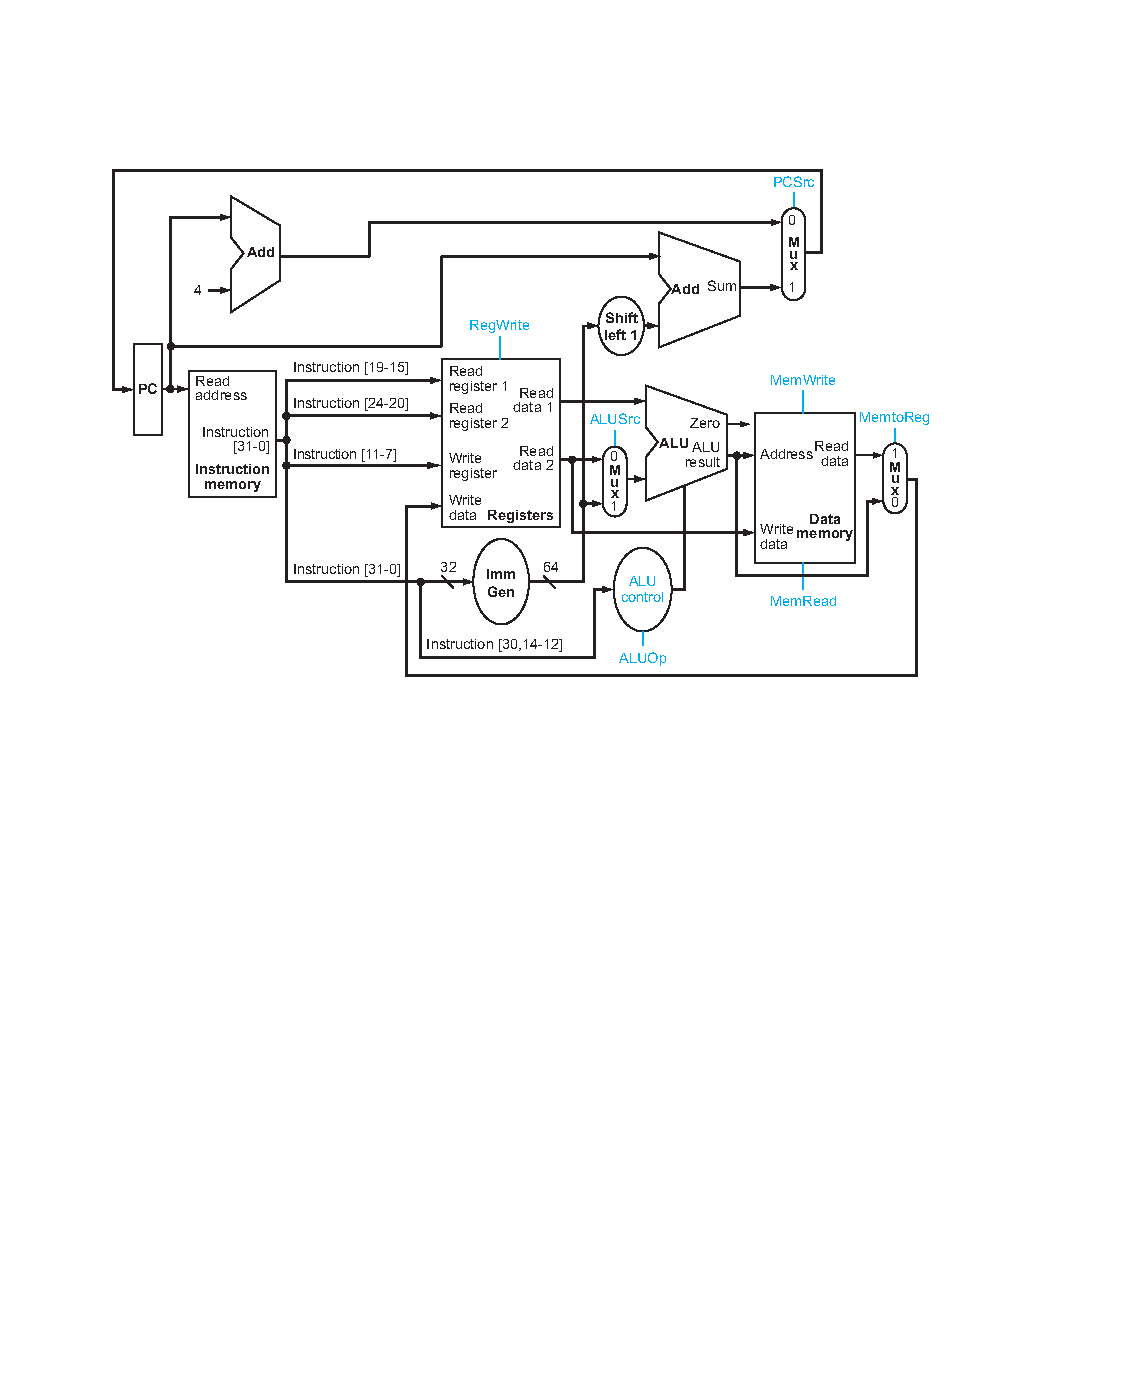
\includegraphics{fig1.pdf}
	\caption{单周期CPU概要原理图\cite{ref1}}
	\label{fig:label1}
\end{figure}

此外,{\tt ctrl\_encode\_def.v}文件进行各类控制信号和指令内容的宏定义,{\tt sccomp\_tb.v}中存放测试文件,进行仿真时的控制和调试。

\subsection{PC(程序计数器)}

\subsubsection{功能描述}

	根据输入信号(包括输入数据以及控制信号)输出程序需要执行的指令地址,并向IM(指令存储器)输出这个地址。该值在每个指令周期用NPC模块的输出进行更新。

\subsubsection{模块接口}
	\begin{center}

	
	\begin{tabular}{|c|c|c|}
		\hline
		信号名&方向&描述\\
		\hline
		{\tt clk}&input&时钟信号\\
		\hline
		{\tt rst}&input&复位信号\\
		\hline
		{\tt NPC}&input&来自{\tt NPC}模块的控制下一PC的输入\\
		\hline
		{\tt PC}&output&输出的PC信号\\
		\hline
	\end{tabular}

	\end{center}

\subsection{RF(寄存器文件)}

\subsubsection{功能描述}

	控制32个寄存器的读写操作。在任意时刻都可以根据输入{\tt A1[4:0]}和{\tt A2[4:0]}的值读取指定编号的寄存器的值,并赋值给{\tt RD1[31:0]},{\tt RD2[31:0]}作为输出。当时钟处在上升沿时,并且写寄存器信号{\tt RFWr}有效,由{\tt A3[4:0]}的值决定向指定编号的寄存器写入{\tt WD[31:0]}的值。

\subsubsection{模块接口}

	\begin{center}
		
		
		\begin{tabular}{|c|c|c|}
			\hline
			信号名&方向&描述\\
			\hline
			{\tt clk}&input&时钟信号\\
			\hline
			{\tt rst}&input&复位信号\\
			\hline
			{\tt RFWr}&input&寄存器写信号\\
			\hline
			{\tt A1[4:0]}&input&读寄存器的第一个地址\\
			\hline
			{\tt A2[4:0]}&input&读寄存器的第二个地址\\
			\hline
			{\tt A3[4:0]}&input&写寄存器的地址\\
			\hline
			{\tt WD[31:0]}&input&写入寄存器的数据\\
			\hline
			{\tt RD1[31:0]}&output&第一个读寄存器的数据\\
			\hline
			{\tt RD2[31:0]}&output&第二个读寄存器的数据\\
			\hline
		\end{tabular}
		
	\end{center}

\subsection{Ctrl(控制模块)}

\subsubsection{功能描述}

	根据输入的指令,控制其他模块的使能信号和选择信号。

\subsubsection{模块接口}

\begin{center}
	
	
	\begin{tabular}{|c|c|c|}
		\hline
		信号名&方向&描述\\
		\hline
		{\tt Op[6:0]}&input&指令中第[6:0]位\\
		\hline
		{\tt Funct7[6:0]}&input&指令中第[31:25]位\\
		\hline
		{\tt Funct3[2:0]}&input&指令中第[14:12]位\\
		\hline
		{\tt Zero}&input&运算单元是否输出为0\\
		\hline
		{\tt RegWrite}&output&寄存器写使能\\
		\hline
		{\tt MemWrite}&output&数据存储器写使能\\
		\hline
		{\tt EXTOp[5:0]}&output&符号扩展运算信号\\
		\hline
		{\tt ALUOp[4:0]}&output&运算单元运算信号\\
		\hline
		{\tt NPCOp[2:0]}&output&控制下一地址模块运算信号\\
		\hline
		{\tt ALUSrc}&output&运算单元来源选择器信号\\
		\hline
		{\tt DMType[2:0]}&output&选择数据存储器访问时的位数\\
		\hline
		{\tt GPRSel[1:0]}&output&备用,无特殊功能\\
		\hline
		{\tt WDSel[1:0]}&output&选择写入寄存器的内容\\
		\hline
	\end{tabular}

\end{center}

\subsection{ALU(运算单元)}

\subsubsection{功能描述}

根据输入的信号,将输入的两个数进行运算得到结果后输出。

\subsubsection{模块接口}

\begin{center}
	
	
	\begin{tabular}{|c|c|c|}
		\hline
		信号名&方向&描述\\
		\hline
		{\tt {\color{gray}signed} A[31:0]}&input&需要运算的第一个数\\
		\hline
		{\tt {\color{gray}signed} B[31:0]}&input&需要运算的第二个数\\
		\hline
		{\tt ALUOp[4:0]}&input&控制运算类型的信号\\
		\hline
		{\tt PC[31:0]}&input&传入当前{\tt PC}信号,便于调试\\
		\hline
		{\tt {\color{gray}signed} C[31:0]}&output&运算后输出的结果\\
		\hline
		{\tt Zero}&output&运算结果是否为0\\
		\hline
	\end{tabular}

\end{center}

\subsection{EXT(符号扩展)}

\subsubsection{功能描述}

根据输入的信号,将输入的立即数进行移位或符号扩展运算得到结果后输出到运算单元或NPC单元。

\subsubsection{模块接口}

\begin{center}
	
	
	\begin{tabular}{|c|c|c|}
		\hline
		信号名&方向&描述\\
		\hline
		{\tt iimm\_shamt[4:0]}&input&指令中第[24:20]位,用于特殊的I型指令\\
		\hline
		{\tt iimm[11:0]}&input&指令中第[31:20]位,用于I型指令\\
		\hline
		{\tt simm[11:0]}&input&指令中第[31:25, 11:7]位,用于S型指令\\
		\hline
		{\tt bimm[11:0]}&input&指令中第[31, 7, 30:25, 11:8]位,用于SB型指令\\
		\hline
		{\tt uimm[19:0]}&input&指令中第[31:12]位,用于U型指令\\
		\hline
		{\tt jimm[19:0]}&input&指令中第[31, 19:12, 20, 30:21]位,用于J型指令\\
		\hline
		{\tt EXTOp[5:0]}&input&控制EXT模块运算类型\\
		\hline
		{\tt immout[31:0]}&output&EXT模块的输出结果\\
		\hline
	\end{tabular}
	
\end{center}

\subsection{DM(数据存储器)}

\subsubsection{功能描述}

根据输入的信号和指令,将相应内存地址的数据写入或取出。写入只在时钟上升沿发生,取出可以是任意时候的。同时也支持取出低1字节、低2字节、低4字节。数据在内存中用小端法存储,一个地址储存1个字节的数据。内存中预置了512个字节空间。在具体结合SoC系统在Xilinx ISE中实现时,没有该部分。

\subsubsection{模块接口}

\begin{center}
	
	
	\begin{tabular}{|c|c|c|}
		\hline
		信号名&方向&描述\\
		\hline
		{\tt clk}&input&时钟信号\\
		\hline
		{\tt DMWr}&input&写使能信号\\
		\hline
		{\tt addr[8:0]}&input&需要访问的地址\\
		\hline
		{\tt din[31:0]}&input&需要输入的数据\\
		\hline
		{\tt DMType[2:0]}&input&控制输入/取出数据的字节数\\
		\hline
		{\tt dout[31:0]}&output&从访问地址读出的数据\\
		\hline
	\end{tabular}

\end{center}

\subsection{IM(指令存储器)}

\subsubsection{功能描述}

根据输入的信号和地址,将相应指令地址的数据取出,送往后续控制器等模块。在具体结合SoC系统在Xilinx ISE中实现时,没有该部分。

\subsubsection{模块接口}

\begin{center}
	
	
	\begin{tabular}{|c|c|c|}
		\hline
		信号名&方向&描述\\
		\hline
		{\tt addr[8:2]}&input&输入的指令地址\\
		\hline
		{\tt dout[31:0]}&output&从指令地址读出的数据\\
		\hline
	\end{tabular}
\end{center}

\subsection{NPC(下一指令地址)}

\subsubsection{功能描述}

根据输入的信号、输入的立即数和当前指令地址PC,计算下一指令地址,在下一时钟周期送往PC计数器。

\subsubsection{模块接口}

\begin{center}
	
	
	\begin{tabular}{|c|c|c|}
		\hline
		信号名&方向&描述\\
		\hline
		{\tt PC[31:0]}&input&当前的指令地址\\
		\hline
		{\tt NPCOp[2:0]}&input&选择下一指令地址的控制信号\\
		\hline
		{\tt IMM[31:0]}&input&输入的立即数\\
		\hline
		{\tt aluout[31:0]}&input&当前运算单元的输出\\
		\hline
		{\tt NPC[31:0]}&output&下一时钟周期的PC地址\\
		\hline
	\end{tabular}
\end{center}

\newpage

\section{详细设计 - 单周期}

\subsection{CPU总体结构}

依据教材《计算机组成与设计:软/硬件接口 RISC-V(第五版)》\cite{ref1}中单周期架构CPU各模块的输入、输出端口,功能信号的规定以及RISC-V指令集中各个指令对应的数据周转流程与对应信号。模块中所有连线基于该架构进行实现。

\begin{figure}[ht]
	\centering
	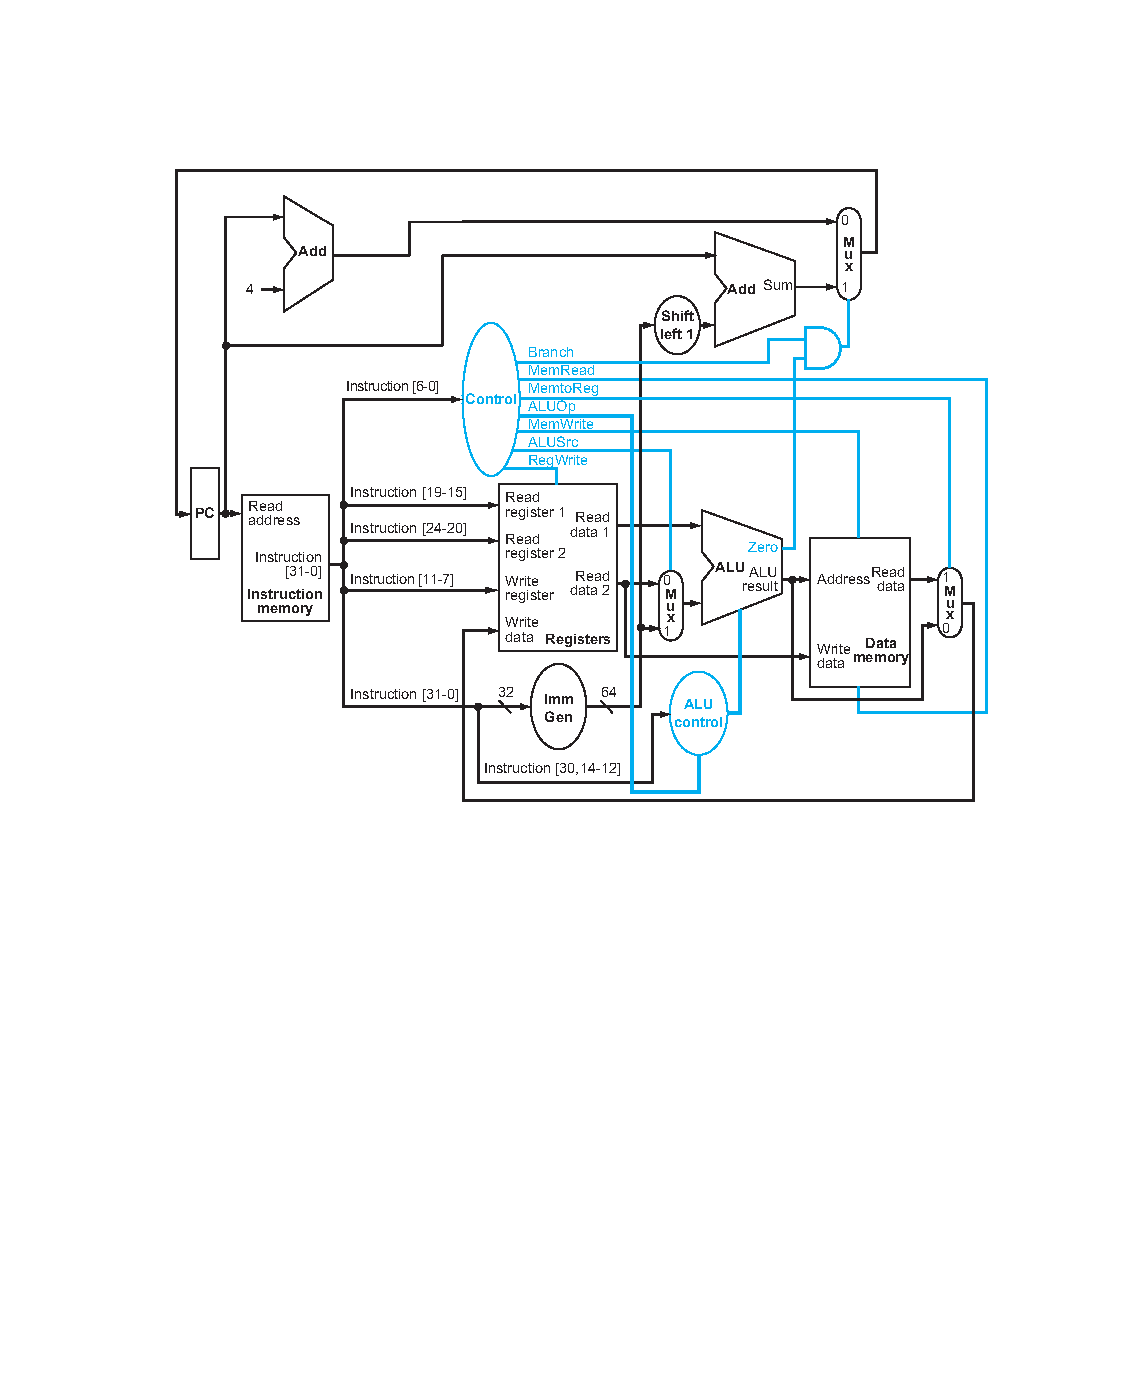
\includegraphics{fig2.pdf}
	\caption{单周期CPU原理图\cite{ref1}}
	\label{fig:label2}
\end{figure}

用 {\tt SCPU.v} 文件将Ctrl、PC、NPC、EXT、RF、ALU整合到同一文件中;然后再用{\tt sccomp.v}挂载DM、IM文件和SCPU进行交互。

此处将DM、IM文件独立的原因是:在SoC系统中,DM和IM分别用Xilinx ISE内置的IP core,预置内容后直接按要求导入模块。

{\tt SCPU.v}设计如下:(省略连线,详见附件中{\tt .v}文件)

{\lstset{language=verilog}\zihao{5}
\begin{lstlisting}
`include "ctrl_encode_def.v"
module SCPU(
	input      clk,          // 时钟信号
	input      reset,        // 复位信号
	input [31:0]  inst_in,   // 输入指令
	input [31:0]  Data_in,   // 来自 DM 的数据

	output    mem_w,        // DM 写使能
	output [31:0] PC_out,   // 输出 PC 地址( debug 用)

	output [31:0] Addr_out, // ALU 输出值(一般用于计算地址)
	output [31:0] Data_out, // 输入 DM 的数据
	output [2:0] DMType     // 选择访问 DM 的字节数
);
	assign Addr_out=aluout;
	assign B = (ALUSrc) ? immout : RD2; // ALU 第二个操作数的来源
	assign Data_out = RD2;
	
	assign iimm_shamt=inst_in[24:20]; //UJ 型指令
	assign iimm=inst_in[31:20];  //I 型指令
	assign simm={inst_in[31:25],inst_in[11:7]}; //S 型指令
	assign bimm={inst_in[31],inst_in[7],inst_in[30:25],inst_in[11:8]};  //SB 型
	assign uimm=inst_in[31:12];  //U 型
	assign jimm={inst_in[31],inst_in[19:12],inst_in[20],inst_in[30:21]};  //J 型
	
	assign Op = inst_in[6:0];  // opcode 部分
	assign Funct7 = inst_in[31:25]; // funct7 部分
	assign Funct3 = inst_in[14:12]; // funct3 部分
	assign rs1 = inst_in[19:15];  // rs1 序号
	assign rs2 = inst_in[24:20];  // rs2 序号
	assign rd = inst_in[11:7];  // rd 序号
	assign Imm12 = inst_in[31:20];
	assign IMM = inst_in[31:12];
	
	// 各模块的例化
	ctrl U_ctrl(.Op(Op), .Funct7(Funct7), .Funct3(Funct3), .Zero(Zero), .RegWrite(RegWrite), .MemWrite(mem_w),
		.EXTOp(EXTOp), .ALUOp(ALUOp), .NPCOp(NPCOp), 
		.ALUSrc(ALUSrc), .GPRSel(GPRSel), .WDSel(WDSel), .DMType(DMType) );
	PC U_PC(.clk(clk), .rst(reset), .NPC(NPC), .PC(PC_out) );
	NPC U_NPC(.PC(PC_out), .NPCOp(NPCOp), .IMM(immout), .NPC(NPC), .aluout(aluout) );
	EXT U_EXT(.iimm_shamt(iimm_shamt), .iimm(iimm), .simm(simm), .bimm(bimm), .uimm(uimm), .jimm(jimm),
	.EXTOp(EXTOp), .immout(immout) );
	RF U_RF(.clk(clk), .rst(reset), .RFWr(RegWrite), 
	.A1(rs1), .A2(rs2), .A3(rd), //Read1, Read2, Write
	.WD(WD), //Write data
	.RD1(RD1), .RD2(RD2) //Read1 Read2
	);
	alu U_alu(.A(RD1), .B(B), .ALUOp(ALUOp), .C(aluout), .Zero(Zero), .PC(PC_out) );
always @*
begin
	case(WDSel)
		`WDSel_FromALU: WD<=aluout;
		`WDSel_FromMEM: WD<=Data_in;
		`WDSel_FromPC: WD<=PC_out+4;
	endcase
end
endmodule
\end{lstlisting}}

{\tt sccomp.v} 设计如下:(省略连线,详见附件中{\tt .v}文件)

{\lstset{language=verilog}\zihao{5}
	\begin{lstlisting}
module sccomp(clk, rstn, reg_sel, reg_data);
	input          clk;
	input          rstn;
	input [4:0]    reg_sel;
	output [31:0]  reg_data;

// CPU 除存储器外部分的例化
SCPU U_SCPU(.clk(clk), .reset(rst), .inst_in(instr), .Data_in(dm_dout),
	.mem_w(MemWrite), .PC_out(PC), .Addr_out(dm_addr),
	.Data_out(dm_din), .reg_sel(reg_sel), .reg_data(reg_data), .DMType(DMType) );

// 存储器的例化
dm    U_DM(.clk(clk), DMWr(MemWrite), .addr(dm_addr),
.din(dm_din), .DMType(DMType), .dout(dm_dout) );

im    U_IM (.addr(PC[8:2]), .dout(instr) );
//这里 PC 截掉最低 2 位,保证 PC 总为 4 的倍数

endmodule

\end{lstlisting}}


\subsection{PC(程序计数器)}

{\lstset{language=verilog}\zihao{5}
	\begin{lstlisting}

module PC( clk, rst, NPC, PC );
	input              clk;
	input              rst;
	input       [31:0] NPC;
	output reg  [31:0] PC;

	always @(posedge clk, posedge rst)
	if (rst) //复位信号
		PC <= 32'h0000_0000;
	else
		PC <= NPC;

endmodule

\end{lstlisting}}

\subsection{RF(程序计数器)}

{\lstset{language=verilog}\zihao{5}
	\begin{lstlisting}
		
module RF(  input         clk, 
			input         rst,
			input         RFWr, 
			input  [4:0]  A1, A2, A3, 
			input  [31:0] WD, 
			output [31:0] RD1, RD2);

reg [31:0] rf[31:0];

integer i;

always @(posedge clk, posedge rst)
	if (rst) begin    // 初始化
		for (i=1; i<32; i=i+1)
			rf[i] <= 0; //  i;
		end

	else 
	if (RFWr&&A3) begin
		rf[A3] <= WD;
	//        $display("r[00-07]=0x%8X, 0x%8X, 0x%8X, 0x%8X, 0x%8X, 0x%8X, 0x%8X, 0x%8X", 0, rf[1], rf[2], rf[3], rf[4], rf[5], rf[6], rf[7]);
	//    此处做 debug 用,省略其他 display 语句
	end
	
	assign RD1 = (A1 != 0) ? rf[A1] : 0;
	assign RD2 = (A2 != 0) ? rf[A2] : 0;

endmodule 
		
\end{lstlisting}}

\subsection{Ctrl(控制模块)}

	Ctrl 根据预置的控制信号,如表\ref{fig:label3}所示,依据输入的指令进行相应类型判断和信号输出。
	
	附件中 {\tt ctrl\_encode\_def.v} 也依照下表进行定义。
	
	\begin{figure}[hp]
		\centering
		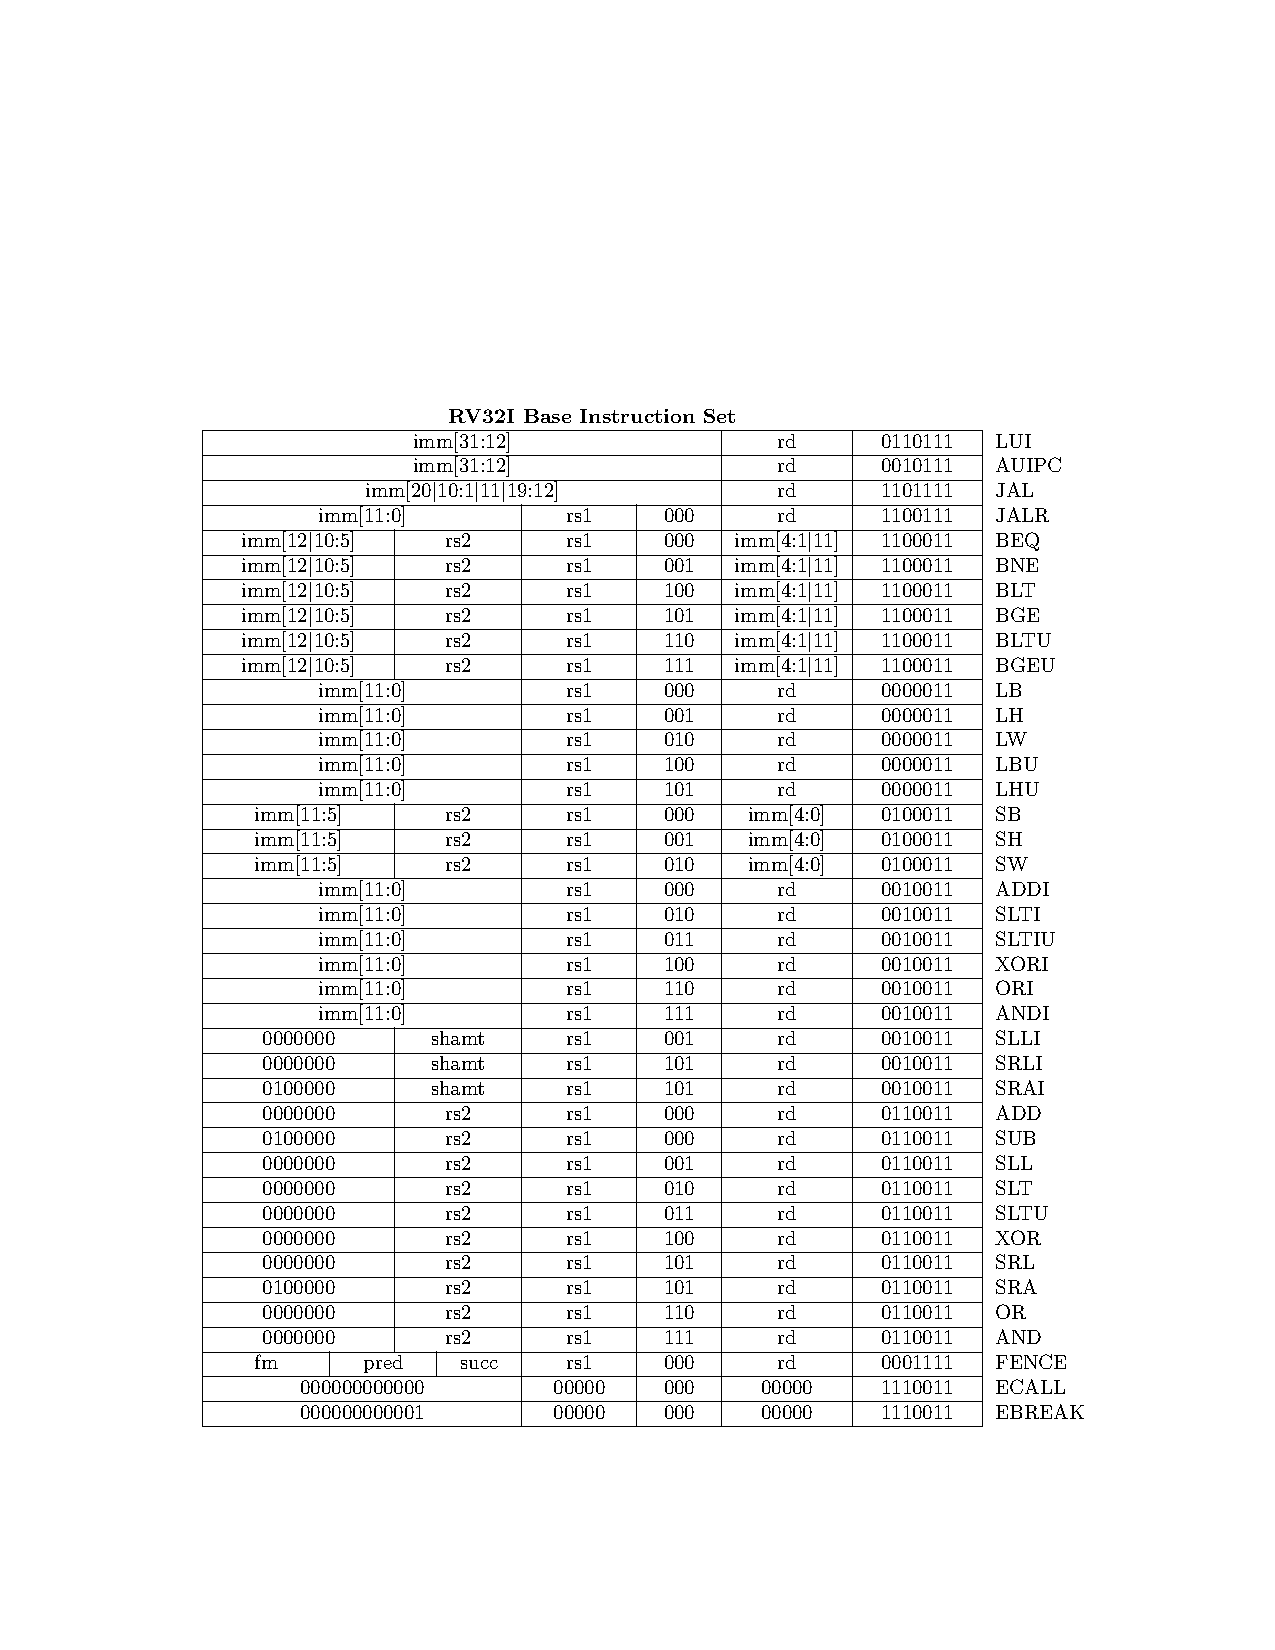
\includegraphics{riscv.pdf}
		\caption{RISC-V指令集}
		\label{fig:label3}
	\end{figure}

\newpage
	   
{\lstset{language=verilog}\zihao{5}
	\begin{lstlisting}
module ctrl(Op, Funct7, Funct3, Zero, RegWrite, MemWrite, EXTOp, ALUOp, NPCOp, ALUSrc, GPRSel, WDSel,DMType );

	input  [6:0] Op;      // opcode
	input  [6:0] Funct7;  
	input  [2:0] Funct3;  
	input        Zero;	  // 运算器输出是否为 0
	
	output       RegWrite; // 寄存器写使能
	output       MemWrite; // 存储器写使能
	output [5:0] EXTOp;    // 符号扩展控制信号
	output [4:0] ALUOp;    // 运算器控制信号
	output [2:0] NPCOp;    // NPC 控制信号
	output       ALUSrc;   // 运算器输入选择信号
	output [2:0] DMType;   // 存储器字节数选择信号

	// 省略根据指令判断类型部分代码,具体依照表 3 进行判断

	// 根据指令类型输出相应信号
	assign RegWrite   = rtype | itype_l | itype_r | i_jalr | i_jal | i_lui | i_auipc;
	assign MemWrite   = stype;     
	assign ALUSrc     = itype_l | itype_r | stype | i_jal | i_jalr | i_auipc | i_lui;  
	
	assign EXTOp[5] = i_slli | i_srli | i_srai;
	assign EXTOp[4] =  itype_l | i_addi | i_slti | i_sltiu | i_xori | i_ori | i_andi | i_jalr;  
	assign EXTOp[3] = stype; 
	assign EXTOp[2] = sbtype; 
	assign EXTOp[1] = i_auipc|i_lui;   
	assign EXTOp[0] = i_jal;         

	assign DMType[0] = i_lb|i_lh|i_sb|i_sh;
	assign DMType[1] = i_lhu|i_lb|i_sb;
	assign DMType[2] = i_lbu;
	
	assign WDSel[0] = itype_l;
	assign WDSel[1] = i_jal | i_jalr;
	
	assign NPCOp[0] = sbtype & Zero;
	assign NPCOp[1] = i_jal;
	assign NPCOp[2]=i_jalr;
	
	//控制运算器的运算符
	assign ALUOp[0] = i_jal|i_jalr|itype_l|stype|i_addi|i_ori|i_add|i_or|i_bne|i_bge|i_bgeu|i_sltiu|i_sltu|i_slli|i_sll|i_sra|i_srai|i_lui;
	assign ALUOp[1] = i_jal|i_jalr|itype_l|stype|i_addi|i_add|i_and|i_andi|i_auipc|i_blt|i_bge|i_slt|i_slti|i_sltiu|i_sltu|i_slli|i_sll;
	assign ALUOp[2] = i_andi|i_and|i_ori|i_or|i_beq|i_sub|i_bne|i_blt|i_bge|i_xor|i_xori|i_sll|i_slli;
	assign ALUOp[3] = i_andi|i_and|i_ori|i_or|i_bltu|i_bgeu|i_slt|i_slti|i_sltiu|i_sltu|i_xor|i_xori|i_sll|i_slli;
	assign ALUOp[4] = i_srl|i_sra|i_srli|i_srai;

endmodule
		
\end{lstlisting}}

\subsection{ALU(运算单元)}

{\lstset{language=verilog}\zihao{5}
	\begin{lstlisting}
`include "ctrl_encode_def.v"
module alu(A, B, ALUOp, C, Zero,PC);
	input  signed [31:0] A, B;
	input         [4:0]  ALUOp;
	input [31:0] PC;
	output signed [31:0] C;
	output Zero;

	reg [31:0] C;//输出值暂存在寄存器里

	always @( * ) begin
	case ( ALUOp )
		`ALUOp_nop:C=A;
		`ALUOp_lui:C=B;
		`ALUOp_auipc:C=PC+B;
		`ALUOp_add:C=A+B;
		`ALUOp_sub:C=A-B;
		`ALUOp_bne:C={31'b0,(A==B)};
		`ALUOp_blt:C={31'b0,(A>=B)};
		`ALUOp_bge:C={31'b0,(A<B)};
		`ALUOp_bltu:C={31'b0,($unsigned(A)>=$unsigned(B))};
		// 备注:无符号类型需要先将 wire 转为 unsigned
		`ALUOp_bgeu:C={31'b0,($unsigned(A)<$unsigned(B))};
		`ALUOp_slt:C={31'b0,(A<B)};
		`ALUOp_sltu:C={31'b0,($unsigned(A)<$unsigned(B))};
		`ALUOp_xor:C=A^B;
		`ALUOp_or:C=A|B;
		`ALUOp_and:C=A&B;
		`ALUOp_sll:C=A<<B;
		`ALUOp_srl:C=A>>B;
		`ALUOp_sra:C=A>>>B;
	endcase
	end

	assign Zero = (C == 32'b0);

endmodule

\end{lstlisting}}
	

\subsection{EXT(符号扩展)}

{\lstset{language=verilog}\zihao{5}
	\begin{lstlisting}
`include "ctrl_encode_def.v"
module EXT( 
	input [4:0] iimm_shamt,
	input	[11:0]		iimm,
	input	[11:0]		simm,
	input	[11:0]		bimm,
	input	[19:0]		uimm,
	input	[19:0]		jimm,
	input	[5:0]		EXTOp,
	output	reg [31:0]  immout);

	always  @(*)
	case (EXTOp)
	  `EXT_CTRL_ITYPE_SHAMT:   immout<={27'b0,iimm_shamt[4:0]};
	  `EXT_CTRL_ITYPE: immout<={{{32-12}{iimm[11]}}, iimm[11:0]};
	  `EXT_CTRL_STYPE: immout<={{{32-12}{simm[11]}}, simm[11:0]};
	  `EXT_CTRL_BTYPE: immout<={{{32-13}{bimm[11]}}, bimm[11:0], 1'b0}; 
	  //忽略最低位,即乘 2 ,下同
	  `EXT_CTRL_UTYPE: immout<={uimm[19:0], 12'b0}; 
	  `EXT_CTRL_JTYPE: immout<={{{32-21}{jimm[19]}}, jimm[19:0], 1'b0};
  	  default:	       immout<=32'b0;
	endcase

endmodule
		
\end{lstlisting}}
\subsection{NPC(下一指令地址)}
{\lstset{language=verilog}\zihao{5}
	\begin{lstlisting}
`include "ctrl_encode_def.v"

module NPC(PC, NPCOp, IMM, NPC,aluout);

	input  [31:0] PC;  
	input  [2:0]  NPCOp;
	input  [31:0] IMM;
	input [31:0] aluout;
	output reg [31:0] NPC;
	
	wire [31:0] PCPLUS4;
	
	assign PCPLUS4 = PC + 4;
	
	//根据不同控制信号进行下一 PC 指令的选择和计算
	
	always @(*) begin
	case (NPCOp)
		`NPC_PLUS4:  NPC = PCPLUS4;
		`NPC_BRANCH: NPC = PC+IMM;
		`NPC_JUMP:   NPC = PC+IMM;
		`NPC_JALR:	NPC =aluout;
		default:     NPC = PCPLUS4;
	endcase
	end

endmodule
\end{lstlisting}}

\section{概要设计 - 流水线}

\subsection{总体设计}

流水线CPU由DM(数据存储器)、IM(指令存储器)、RF(寄存器文件)、PC(程序计数器)、EXT(符号扩展)、ALU(运算单元)、Ctrl(控制模块)等部分组成,此外,将EXT、流水线寄存器、冒险探测、旁路选择等模块单独放在{\tt parts.v}文件中。PC、EXT、ALU、RF、流水线寄存器和冒险处理综合在{\tt datapath.v}文件中;Ctrl单独作为文件{\tt controller.v}进行定义;DM、IM作为存储器,独立于CPU文件,作为Xilinx ISE的IP core进行连线。

\begin{figure}[h]
	\centering
	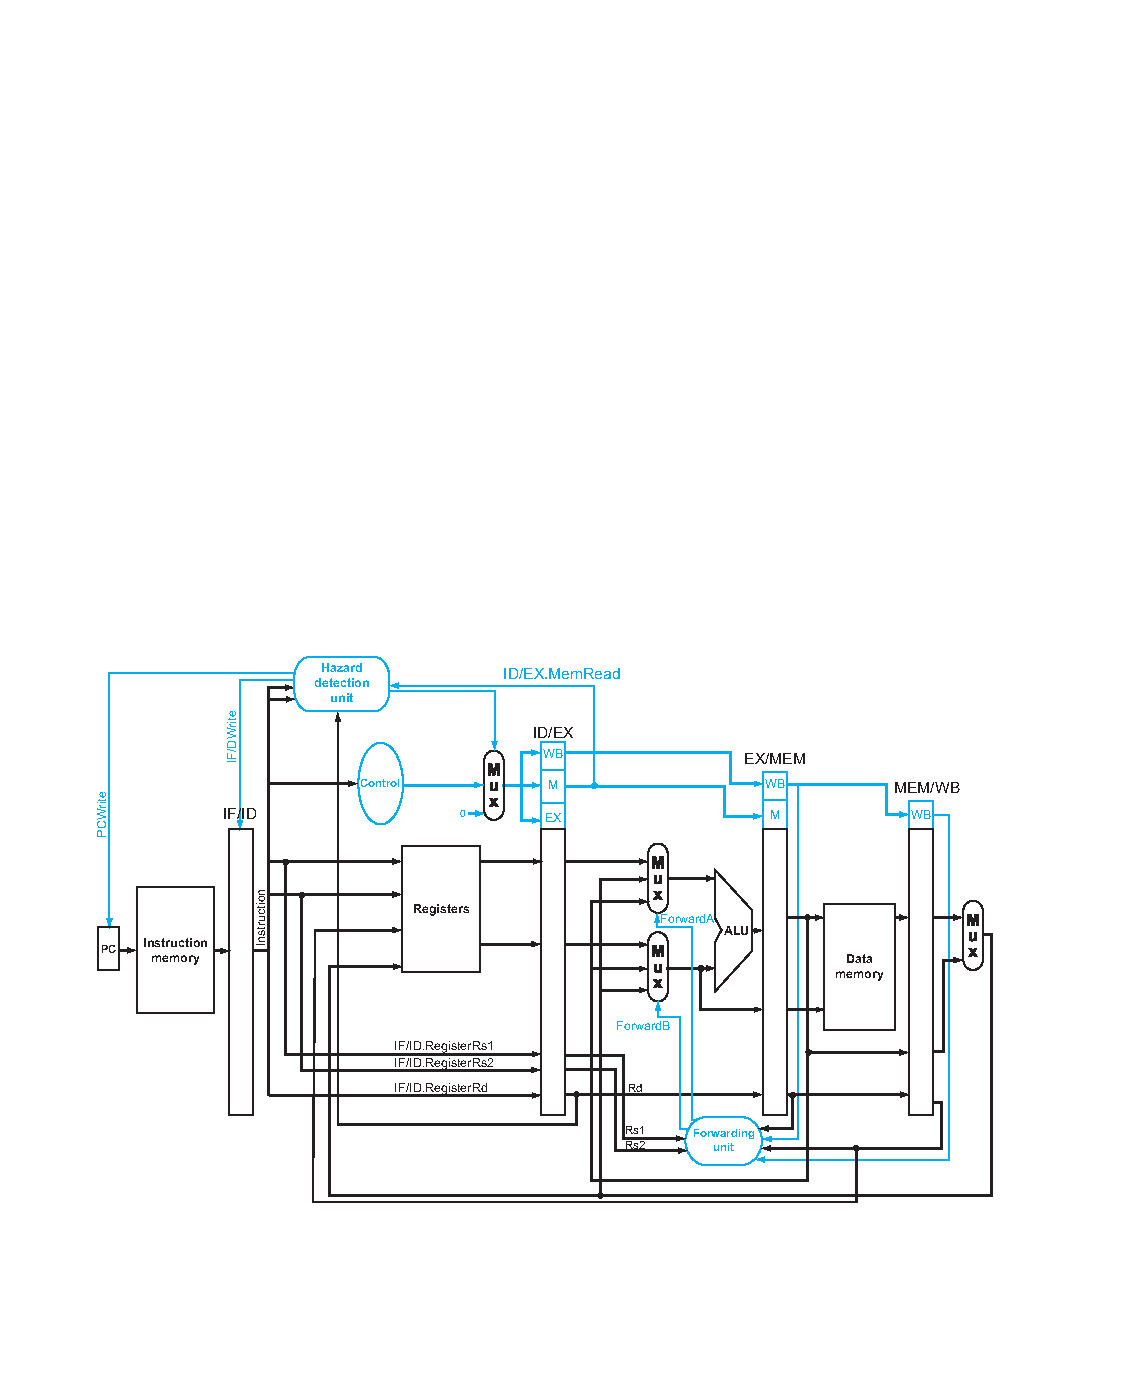
\includegraphics{fig4.pdf}
	\caption{流水线CPU概要原理图\cite{ref1}}
	\label{fig:label4}
\end{figure}

流水线被划分为 IF(取指), ID(译码), EX(运算), MEM(访存), WB(写回)五个部分,每两个部分之间由流水线寄存器暂时存放数据。同时为了防止冒险,引入冒险探测、旁路选择,并实现了控制冒险的阻塞。由于同时存在DM和IM,不会存在结构冒险。

此外,{\tt xgriscv\_defines.v}文件进行各类控制信号和指令内容的宏定义。

\subsection{PC(程序计数器)}

\subsubsection{功能描述}

根据输入信号(包括输入数据以及控制信号)输出程序需要执行的指令地址,并向IM(指令存储器)输出这个地址。该值在每个指令周期根据控制信号更新为PC$+4$或其他跳转后信号。

\subsubsection{模块接口}
\begin{center}
	
	
	\begin{tabular}{|c|c|c|}
		\hline
		信号名&方向&描述\\
		\hline
		{\tt clk}&input&时钟信号\\
		\hline
		{\tt reset}&input&复位信号\\
		\hline
		{\tt en}&input&使能信号\\
		\hline
		{\tt d}&input&输入作为下一PC的值\\
		\hline
		{\tt q}&output&输出的PC信号\\
		\hline
	\end{tabular}

	
\end{center}

\subsection{RF(寄存器文件)}

\subsubsection{功能描述}

控制32个寄存器的读写操作。在任意时刻都可以根据输入{\tt A1[4:0]}和{\tt A2[4:0]}的值读取指定编号的寄存器的值,并赋值给{\tt RD1[31:0]},{\tt RD2[31:0]}作为输出。当时钟处在上升沿时,并且写寄存器信号{\tt RFWr}有效,由{\tt A3[4:0]}的值决定向指定编号的寄存器写入{\tt WD[31:0]}的值。

\subsubsection{模块接口}

\begin{center}
	\begin{tabular}{|c|c|c|}
		\hline
		信号名&方向&描述\\
		\hline
		{\tt clk}&input&时钟信号\\
		\hline
		{\tt ra1[4:0]}&input&读寄存器的第一个地址\\
		\hline
		{\tt ra2[4:0]}&input&读寄存器的第二个地址\\
		\hline
		{\tt rd1[31:0]}&output&第一个读寄存器的数据\\
		\hline
		{\tt rd2[31:0]}&output&第二个读寄存器的数据\\
		\hline
		{\tt we3}&input&寄存器写使能\\
		\hline
		{\tt wa3[4:0]}&input&写寄存器的地址\\
		\hline
		{\tt wd3[31:0]}&input&写入寄存器的数据\\
		\hline
		{\tt pc[31:0]}&input&PC值(用于debug)\\
		\hline
	\end{tabular}
	
\end{center}

\subsection{Ctrl(控制模块)}

\subsubsection{功能描述}

根据输入的指令,控制其他模块的使能信号和选择信号。

\subsubsection{模块接口}

\begin{center}
	
	\begin{tabular}{|c|c|c|}
		\hline
		信号名&方向&描述\\
		\hline
		{\tt clk}&input&时钟信号\\
		\hline
		{\tt reset}&input&复位信号\\
		\hline
		{\tt opcode[6:0]}&input&指令中第[6:0]位\\
		\hline
		{\tt funct7[6:0]}&input&指令中第[31:25]位\\
		\hline
		{\tt funct3[2:0]}&input&指令中第[14:12]位\\
		\hline
		{\tt rd[4:0]}&input&\multirow{3}*{用于判断{\tt nop}}\\
		\cline{1-2}
		{\tt rs1[4:0]}&input&\\
		\cline{1-2}
		{\tt imm[11:0]}&input&\\
		\hline
		{\tt immctrl[4:0]}&output&控制符号扩展模块运算信号\\
		\hline
		{\tt itype}&output&判断是否为I型指令\\
		\hline
		{\tt jal}&output&判断是否为{\tt jal}指令\\
		\hline
		{\tt jalr}&output&判断是否为{\tt jalr}指令\\
		\hline
		{\tt bunsigned}&output&判断是否为无符号的B型指令\\
		\hline
		{\tt lunsigned}&output&判断是否为无符号的load类I型指令\\
		\hline
		{\tt pcsrc}&output&控制下一个PC信号的来源\\
		\hline
		%%%%%%%%%%
		{\tt aluctrl[3:0]}&output&控制第一个运算单元的运算类型\\
		\hline
		{\tt aluctrl1[2:0]}&output&控制第二个运算单元的运算类型\\
		\hline
		{\tt alusrca[1:0]}&output&控制第一个数的来源\\
		\hline
		{\tt alusrcb}&output&控制第二个数的来源\\
		\hline
		{\tt j}&output&判断是否为J型指令\\
		\hline
		{\tt btype}&output&判断是否为SB型指令\\
		\hline
		{\tt lwhb}&output&load类指令的word, half, byte判断\\
		\hline
		{\tt swhb}&output&S型指令的word, half, byte判断\\
		\hline
	\end{tabular}
	
\end{center}

\subsection{ALU(运算单元)}

\subsubsection{功能描述}

根据输入的信号,将输入的两个数进行运算得到结果后输出。为了方便计算跳转后的地址,在数据通路中引用了两个ALU。

\subsubsection{模块接口}

\begin{center}

	\begin{tabular}{|c|c|c|}
		\hline
		信号名&方向&描述\\
		\hline
		{\tt {\color{gray}signed} a[31:0]}&input&需要运算的第一个数\\
		\hline
		{\tt {\color{gray}signed} b[31:0]}&input&需要运算的第二个数\\
		\hline
		{\tt aluctrl[3:0]}&input&控制第一个ALU运算类型的信号\\
		\hline
		{\tt aluctrl1[2:0]}&input&控制第二个ALU运算类型的信号\\
		\hline
		{\tt aluout[31:0]}&output&运算后输出的结果\\
		\hline
		{\tt overflow}&output&运算结果是否发生溢出\\
		\hline
		{\tt zero}&output&运算结果是否为0\\
		\hline
		{\tt lt}&output&是否满足$a<b$\\
		\hline
		{\tt ge}&output&是否满足$a\ge b$\\
		\hline
	\end{tabular}
	
\end{center}

\subsection{EXT(符号扩展)}

\subsubsection{功能描述}

根据输入的信号,将输入的立即数进行移位或符号扩展运算得到结果后输出到运算单元,用作取址或跳转指令。在{\tt part.v}中作为{\tt imm}模块实现。

\subsubsection{模块接口}

\begin{center}
	\begin{tabular}{|c|c|c|}
		\hline
		信号名&方向&描述\\
		\hline
		{\tt iimm[11:0]}&input&指令中第[31:20]位,用于I型指令\\
		\hline
		{\tt simm[11:0]}&input&指令中第[31:25, 11:7]位,用于S型指令\\
		\hline
		{\tt bimm[11:0]}&input&指令中第[31, 7, 30:25, 11:8]位,用于SB型指令\\
		\hline
		{\tt uimm[19:0]}&input&指令中第[31:12]位,用于U型指令\\
		\hline
		{\tt jimm[19:0]}&input&指令中第[31, 19:12, 20, 30:21]位,用于J型指令\\
		\hline
		{\tt immctrl[4:0]}&input&控制EXT模块运算类型\\
		\hline
		{\tt immout[31:0]}&output&EXT模块的输出结果\\
		\hline
	\end{tabular}
	
\end{center}

\subsection{DM(数据存储器)}

\subsubsection{功能描述}

根据输入的信号和指令,将相应内存地址的数据写入或取出。写入只在时钟上升沿发生,取出可以是任意时候的。同时也支持取出低1字节、低2字节、低4字节,Xilinx ISE中预置的IP core可以支持四个字节的任意读写。数据在内存中用小端法存储,一个地址储存4个字节的数据,而汇编指令中一个地址储存1个字节的数据,因此需要在总线中进行转换。内存中预置了1024个字的空间,共4096字节。在具体结合SoC系统在Xilinx ISE中实现时,引用 Block Memory Generator。

\subsubsection{模块接口}

\begin{center}
	
	\begin{tabular}{|c|c|c|}
		\hline
		信号名&方向&描述\\
		\hline
		{\tt clka}&input&时钟信号\\
		\hline
		{\tt WEA[3:0]}&input&每个字节的写使能信号\\
		\hline
		{\tt addra[9:0]}&input&需要访问的字地址\\
		\hline
		{\tt dina[31:0]}&input&需要输入的数据\\
		\hline
		{\tt douta[31:0]}&output&从访问地址读出的数据\\
		\hline
	\end{tabular}
	
\end{center}

\subsection{IM(指令存储器)}

\subsubsection{功能描述}

根据输入的信号和地址,将相应指令地址的数据取出,送往后续控制器等模块。数据在内存中用小端法存储,一个地址储存4个字节的数据,而汇编指令中一个地址储存1个字节的数据,因此需要在总线中进行转换。在具体结合SoC系统在Xilinx ISE中实现时,引用 Distributed Memory Generator。

\subsubsection{模块接口}

\begin{center}
	
	
	\begin{tabular}{|c|c|c|}
		\hline
		信号名&方向&描述\\
		\hline
		{\tt a[9:0]}&input&输入的指令地址\\
		\hline
		{\tt spo[31:0]}&output&从指令地址读出的数据\\
		\hline
	\end{tabular}
\end{center}

\subsection{flop(流水线寄存器)}

\subsubsection{功能描述}

临时存放每个流水线阶段需要传给下个阶段的数据,同时支持复位、写使能、清空,方便插入{\tt nop}指令和执行跳转指令。

\subsubsection{模块接口}

\begin{center}
	\begin{tabular}{|c|c|c|}
		\hline
		信号名&方向&描述\\
		\hline
		{\tt clk}&input&时钟信号\\
		\hline
		{\tt reset}&input&复位信号\\
		\hline
		{\tt en}&input&写入使能信号\\
		\hline
		{\tt clear}&input&清空信号\\
		\hline
		{\tt d[WIDTH-1:0]}&input&输入寄存器的数\\
		\hline
		{\tt q[WIDTH-1:0]}&output&寄存器的输出\\
		\hline
		{\tt WIDTH}&parameter&寄存器位宽参数\\
		\hline
	\end{tabular}
\end{center}

\subsection{hazard(冒险探测)}

\subsubsection{功能描述}

用于对load型指令在MEM阶段才能获取到的数据,需要停顿(阻塞)一个周期才能继续执行。将可能涉及到的数据输入冒险探测模块,即可判断当前状态下各阶段是否需要阻塞。

根据《计算机组成与设计:硬件/软件接口 RISC-V(第五版)》\cite{ref1},如果存在下面这样的数据冒险,则需要停顿:

{\lstset{language=c++}\zihao{5}
	\begin{lstlisting}
if	(ID/EX.MemRead and
	((ID/EX.RegisterRd = IF/ID.RegisterRs1) or
	  (ID/EX.RegisterRd = IF/ID.RegisterRs2)))
	  	stall the pipeline
\end{lstlisting}}

\begin{figure}[ht]
	\centering
	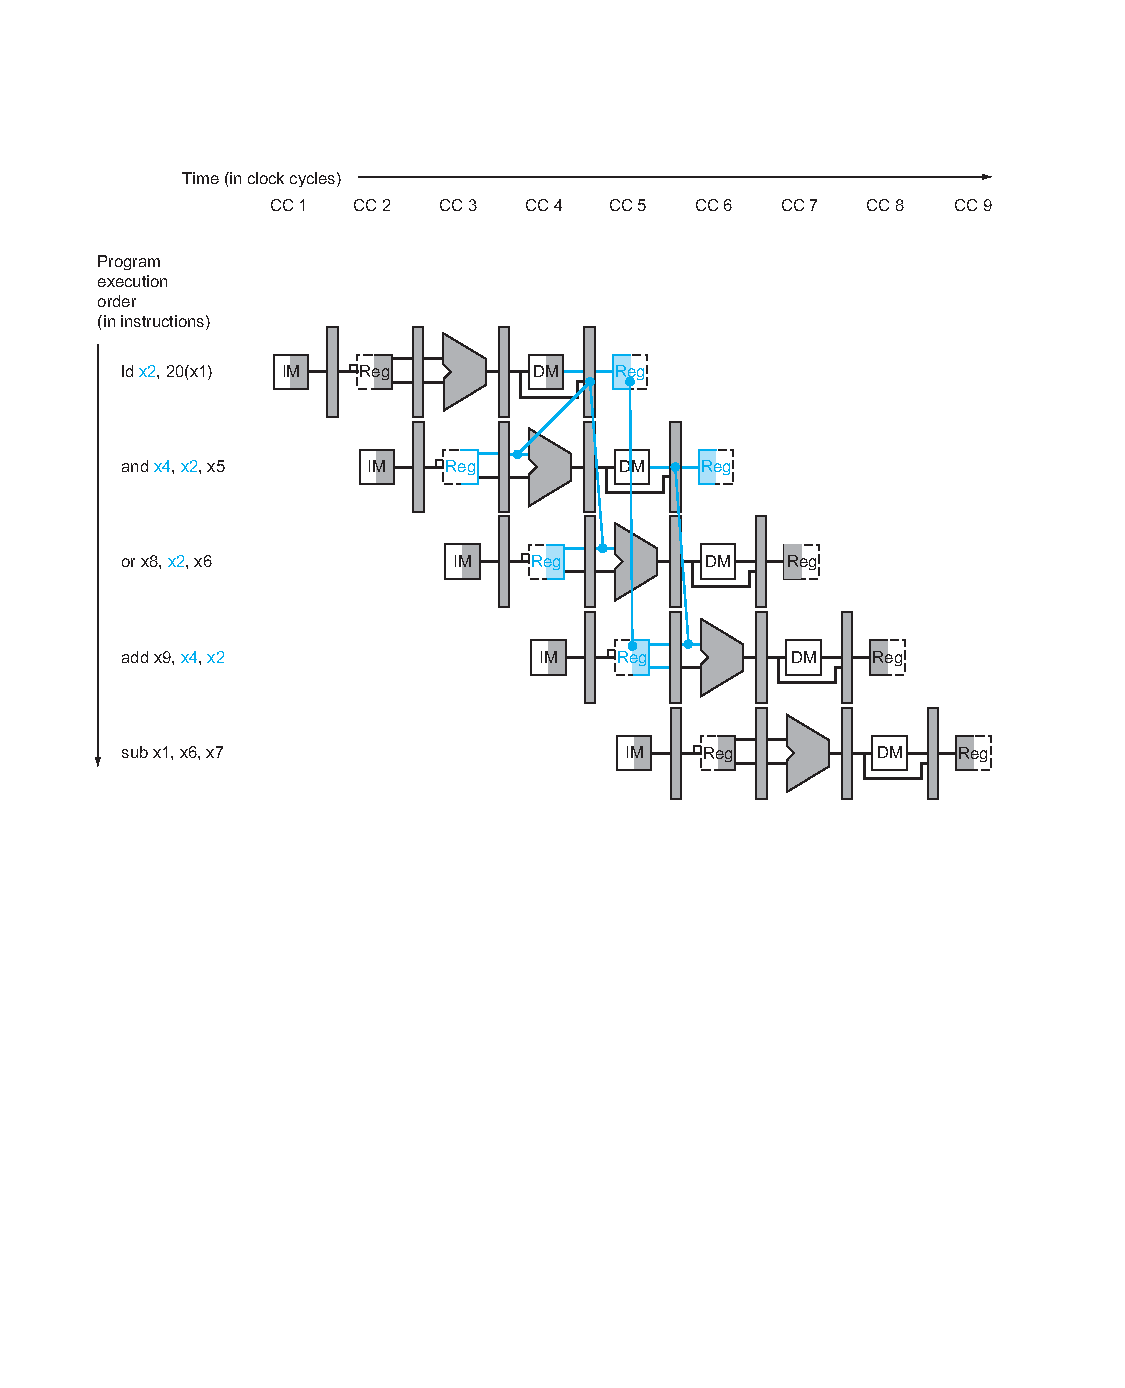
\includegraphics{fig5.pdf}
	\caption{流水线CPU中出现停顿的情况\cite{ref1}}
	\label{fig:label5}
\end{figure}

如果当前正在阻塞,则不进行冒险探测。

\subsubsection{模块接口}

\begin{center}
	\begin{tabular}{|c|c|c|}
		\hline
		信号名&方向&描述\\
		\hline
		{\tt clk}&input&时钟信号\\
		\hline
		{\tt memtoreg}&input&判断此时是否读取存储器\\
		\hline
		{\tt rdE[4:0]}&input&ID/EX阶段的rd序号\\
		\hline
		{\tt rs1D[4:0]}&input&IF/ID阶段的rs1序号\\
		\hline
		{\tt rs2D[4:0]}&input&IF/ID阶段的rs2序号\\
		\hline
		{\tt writenM}&input&上一阶段的阻塞信号\\
		\hline
		{\tt writen}&output&该阶段阻塞信号的输出\\
		\hline
	\end{tabular}
\end{center}

\subsection{forward(旁路前递)}

\subsubsection{功能描述}

对于一些运算指令在流水线中来说,当前的运算的数据可能仍在流水线中进行运算,但多数情况下这样的数据其实已经有了运算结果,处于数据通路中,只是还未写回它应处于的位置。所以要添加旁路前递将这些数据及时取出,以保证流水线架构的正常运作。

根据《计算机组成与设计:硬件/软件接口 RISC-V(第五版)》\cite{ref1},如果存在下面这样的数据冒险,则需要进行旁路前递:

{\lstset{language=c++}\zihao{5}
	\begin{lstlisting}
EX/MEM.RegisterRd = ID/EX.RegisterRs1
EX/MEM.RegisterRd = ID/EX.RegisterRs2
MEM/WB.RegisterRd = ID/EX.RegisterRs1
MEM/WB.RegisterRd = ID/EX.RegisterRs2
\end{lstlisting}}

\begin{figure}[ht]
	\centering
	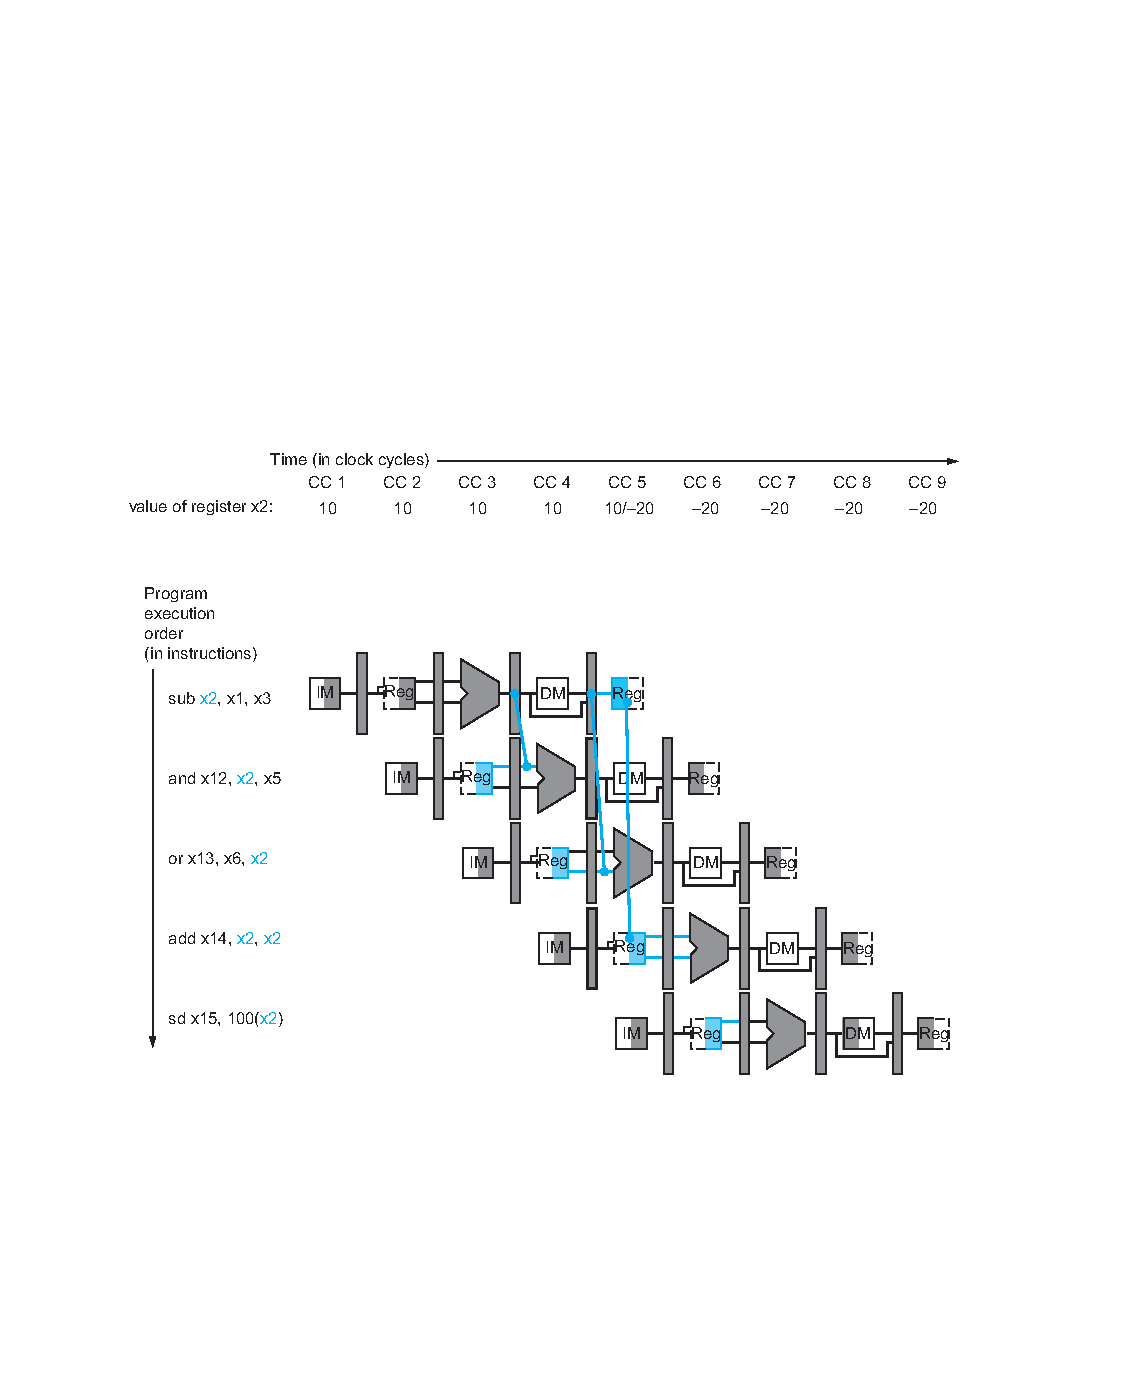
\includegraphics{fig6.pdf}
	\caption{流水线CPU中出现前递的情况\cite{ref1}}
	\label{fig:label6}
\end{figure}

如果当前正在阻塞,则不进行冒险探测。

说明:当{\tt forward}信号为不同值时,对应情况如下\cite{ref1}:

\begin{center}
	\begin{tabular}{|c|c|c|}
		\hline
		控制信号&数据来源&解释\\
		\hline
		$00$&ID/EX&ALU操作数正常来自ID/EX阶段\\
		\hline
		$10$&EX/MEM&ALU操作数从EX/MEM阶段前递过来\\
		\hline
		$01$&MEM/WB&ALU操作数从MEM/WB阶段前递过来\\
		\hline
	\end{tabular}
\end{center}

\subsubsection{模块接口}

\begin{center}
	\begin{tabular}{|c|c|c|}
		\hline
		信号名&方向&描述\\
		\hline
		{\tt regwriteM}&input&EX/MEM阶段的寄存器写使能\\
		\hline
		{\tt rdM[4:0]}&input&EX/MEM阶段的rd序号\\
		\hline
		{\tt rs1E[4:0]}&input&ID/EX阶段的rs1序号\\
		\hline
		{\tt rs2E[4:0]}&input&ID/EX阶段的rs2序号\\
		\hline
		{\tt regwriteW}&input&MEM/WB阶段的寄存器写使能\\
		\hline
		{\tt rdW[4:0]}&input&MEM/WB阶段的rd序号\\
		\hline
		{\tt forwardA[1:0]}&input&旁路A的选择信号\\
		\hline
		{\tt forwardB[1:0]}&input&旁路B的选择信号\\
		\hline
	\end{tabular}
\end{center}

\newpage

\section{详细设计 - 流水线}

\subsection{CPU总体结构}

依据教材《计算机组成与设计:软/硬件接口 RISC-V(第五版)》\cite{ref1}中流水线架构CPU各模块的输入、输出端口,功能信号的规定以及RISC-V指令集中各个指令对应的数据周转流程与对应信号。模块中所有连线基于该架构进行实现。

\begin{figure}[ht]
	\centering
	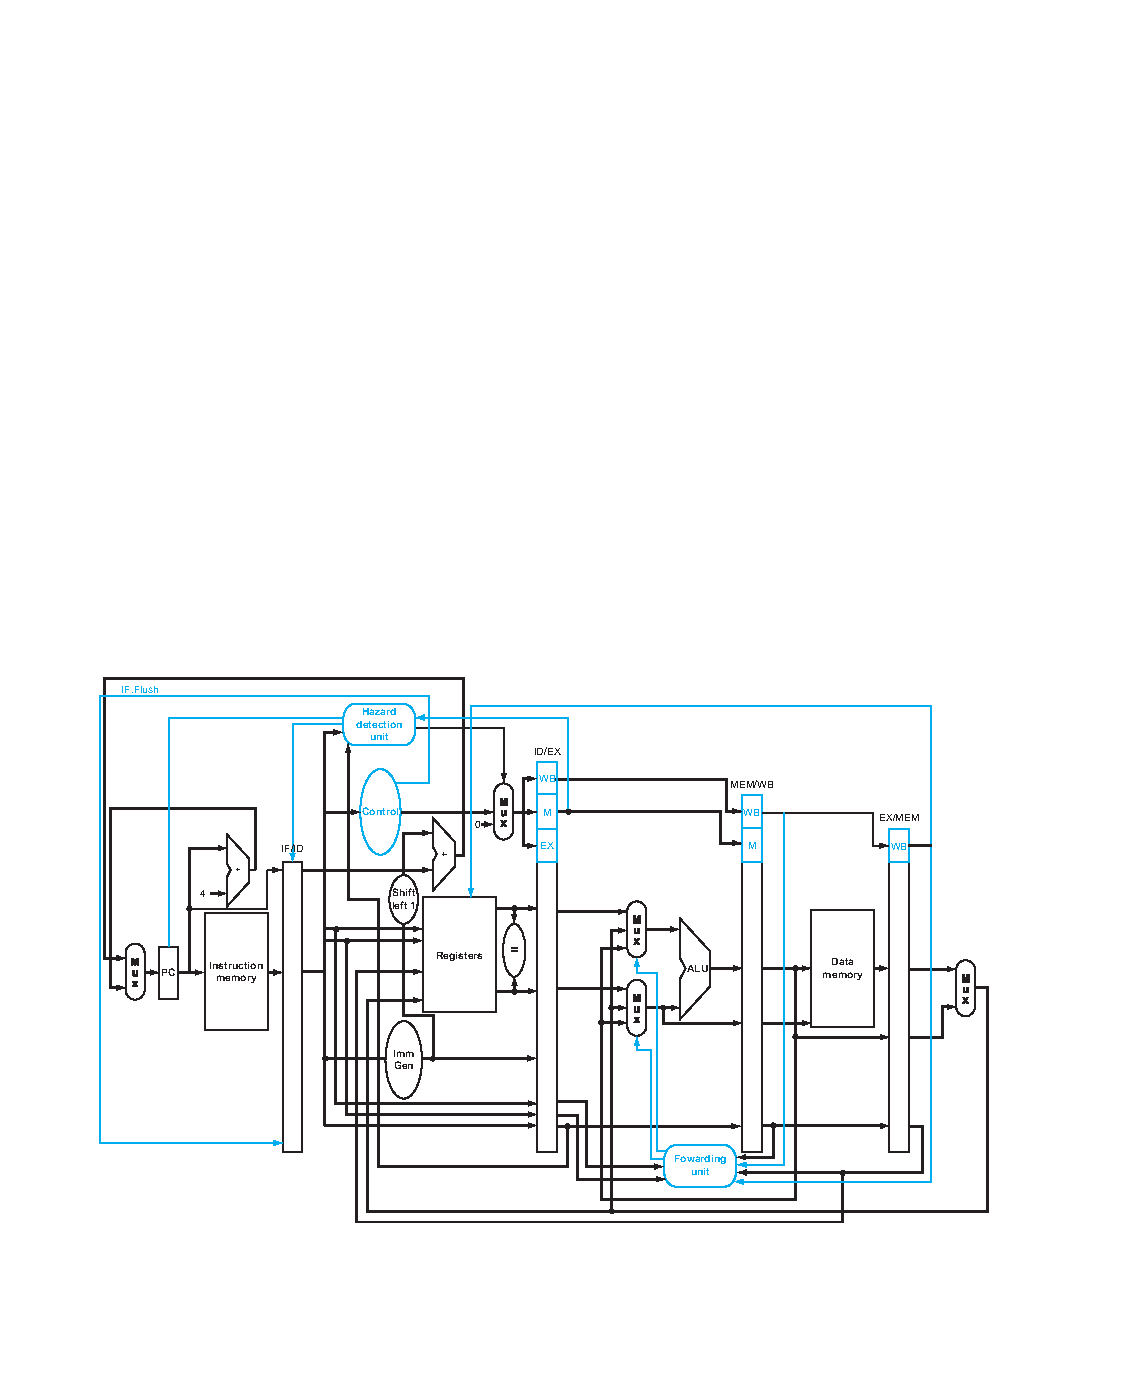
\includegraphics{fig7.pdf}
	\caption{流水线CPU原理图\cite{ref1}}
	\label{fig:label7}
\end{figure}

用 {\tt datapath.v} 文件将PC、EXT、RF、ALU、流水线寄存器和冒险处理等整合到同一文件中;然后再用{\tt pipelined.v}引入Ctrl模块,最终由TOP顶层文件进行组织之后,和封装在IP core的数据存储器(RAM)和指令存储器(ROM)进行交互。并将该文件综合编译为二进制文件比特流后导入SWORD开发板中进行仿真实现并验证。

{\tt pipelined.v}设计如下:(省略连线的声明,详见附件中{\tt .v}文件)

{\lstset{language=verilog}\zihao{5}
	\begin{lstlisting}
`include "xgriscv_defines.v"

//输入输出接口主要用于顶层文件综合
module xgriscv(input  clk, reset,
	input MIO_ready,
	input  [`INSTR_SIZE-1:0] inst_in,
	input  [`XLEN-1:0] Data_in,
	output mem_w,
	output [31:0] PC_out,
	output [`ADDR_SIZE-1:0] 	Addr_out, 
	output [`XLEN-1:0] 		   Data_out,
	output CPU_MIO,
	output[3:0] WEA,
	input INT
	);

	controller  c(clk, reset, opD, funct3D, funct7D, rdD, rs1D, immD, zeroD, ltD,
		immctrlD, itypeD, jalD, jalrD, bunsignedD, pcsrcD, aluctrlD, aluctrl1D, alusrcaD, alusrcbD, memwriteD, lunsignedD, jD, bD, lwhbD, swhbD, memtoregD, regwriteD);
	//Ctrl 部分均为 IF/ID 阶段的信号,因此都标注为 D

	//datapath 在接入 Ctrl 部分的信号后传入数据通路
	datapath    dp(clk, reset, inst_in, PC_out, Data_in, Addr_out, Data_out, mem_w, 
		immctrlD, itypeD, jalD, jalrD, bunsignedD, pcsrcD, aluctrlD, aluctrl1D, alusrcaD, alusrcbD, memwriteD, lunsignedD,  jD, bD, lwhbD, swhbD, memtoregD, regwriteD, 
		opD, funct3D, funct7D, rdD, rs1D, immD, zeroD, ltD, memwriteD, WEA);

endmodule
\end{lstlisting}}

\subsection{datapath(数据通路)}

数据通路中省略无初始化的连线声明,具体见{\tt datapath.v}文件。

{\lstset{language=verilog}\zihao{5}
	\begin{lstlisting}
		
`include "xgriscv_defines.v"

module datapath(
	input                    clk, reset,
	
	input [`INSTR_SIZE-1:0]  instrF,	// from IM
	output[`ADDR_SIZE-1:0] 	 pcF,		// to IM
	
	input [`XLEN-1:0]	     readdataM, // from DM
	output[`XLEN-1:0]        aluoutM, 	// to DM - 地址
	output[`XLEN-1:0]	     writedataM,// to DM - 数据
	output			         memwriteM,	// to DM - 写使能
	
	//控制信号如下
	input [4:0]        immctrlD,
	input			   itype, jalD, jalrD, bunsignedD, pcsrcD,
	input [3:0]		  aluctrlD,
	input [2:0]	      aluctrl1D,
	input [1:0]       alusrcaD,
	input			  alusrcbD,
	input			  memwriteD, lunsignedD, jD, bD,
	input [1:0]		  lwhbD, swhbD,  
	input          	  memtoregD, regwriteD,
	
	//输出到 Ctrl 解析的指令
	output [6:0]	opD,
	output [2:0]	funct3D,
	output [6:0]	funct7D,
	output [4:0] 	rdD, rs1D,
	output [11:0]  	immD,
	output 	       	zeroD, ltD,
	input			data_ram_weD,
	output [3:0]	WEAM );
	wire flushM = 0;
	mux2 #(`ADDR_SIZE)	pcsrcmux(pcplus4F, pcbranchD, pcsrc, nextpcF);
	//PC 寄存器
	pcenr   pcreg(clk, reset, writenE, nextpcF, pcF);
	addr_adder  pcadder1(pcF, `ADDR_SIZE'b100, pcplus4F);
	
	////////////////////////////////////////////////////
	// IF/ID 流水线寄存器
	wire flushD = pcsrc; 

	//分别存储指令、 PC 、 PC+4 的流水线寄存器	
	flopenrc #(`INSTR_SIZE)   pr1D(clk, reset, writenE, flushD, instrF, instrD);     // instruction
	flopenrc #(`ADDR_SIZE)	  pr2D(clk, reset, writenE, flushD, pcF, pcD);           // pc
	flopenrc #(`ADDR_SIZE)	  pr3D(clk, reset, writenE, flushD, pcplus4F, pcplus4D); // pc+4
	
	// Decode stage logic
	assign  opD 	= instrD[6:0];
	assign  rdD     = instrD[11:7];
	assign  funct3D = instrD[14:12];
	assign  rs1D    = instrD[19:15];
	assign  rs2D   	= itype?5'b00000:instrD[24:20];
	//此处如果使用 itype ,则该阶段可能不为 0 (如 srai )
	assign  funct7D = instrD[31:25];
	assign  immD    = instrD[31:20];
	
	//立即数处理部分
	wire [11:0] iimmD = instrD[31:20];
	wire [11:0]	simmD = {instrD[31:25],instrD[11:7]};
	wire [11:0] bimmD = {instrD[31],instrD[7],instrD[30:25],instrD[11:8]};
	wire [19:0]	uimmD = instrD[31:12];
	wire [19:0] jimmD = {instrD[31],instrD[19:12],instrD[20],instrD[30:21]};
	
	imm im(iimmD, simmD, bimmD, uimmD, jimmD, immctrlD, immoutD);
	regfile rf(clk, rs1D, rs2D, rdata1D, rdata2D, regwriteW, waddrW, wdataW, pcW);
	
	////////////////////////////////////////////////////
	// ID/EX 流水线寄存器
	
	// 控制信号寄存器
	assign flushE = pcsrc | ~writenE;
	flopenrc #(21) regE(clk, reset, writenE, flushE, {regwriteD, memwriteD, memtoregD, lwhbD, swhbD, lunsignedD, alusrcaD, alusrcbD, aluctrlD, aluctrl1D, jD, bD, data_ram_weD}, {regwriteE, memwriteE, memtoregE, lwhbE, swhbE, luE, alusrcaE, alusrcbE, aluctrlE, aluctrl1E, jE, bE, data_ram_weE});
	
	// 数据寄存器
	flopenrc #(`XLEN) 	pr1E(clk, reset, writenE, flushE, rdata1D, srca1E);        	// data from rs1
	flopenrc #(`XLEN) 	pr2E(clk, reset, writenE, flushE, rdata2D, srcb1E);         // data from rs2
	flopenrc #(`XLEN) 	pr3E(clk, reset, writenE, flushE, immoutD, immoutE);        // imm output
	flopenrc #(`RFIDX_WIDTH)  pr4E(clk, reset, writenE, flushE, rs1D, rs1E);         // rs1
	flopenrc #(`RFIDX_WIDTH)  pr5E(clk, reset, writenE, flushE, rs2D, rs2E);         // rs2
	flopenrc #(`RFIDX_WIDTH)  pr6E(clk, reset, writenE, flushE, rdD, rdE);         // rd
	flopenrc #(`ADDR_SIZE)	pr8E(clk, reset, writenE, flushE, pcD, pcE);            // pc
	flopenrc #(`ADDR_SIZE)	pr9E(clk, reset, writenE, flushE, pcplus4D, pcplus4E);  // pc+4
	
	wire[1:0]	forwardA, forwardB;
	wire[`XLEN-1:0] srca, srcb;
	mux3 #(`XLEN)	fA(srca1E, wdataW, aluoutM, forwardA, srca);//
	mux3 #(`XLEN)	fB(srcb1E, wdataW, aluoutM, forwardB, srcb);//
	
	// ALU 运算数据来源选择
	mux3 #(`XLEN)  srcamux(srca, 0, pcE, alusrcaE, srcaE);
	mux2 #(`XLEN)  srcbmux(srcb, immoutE, alusrcbE, srcbE);
	
	// 分别用于计算和跳转
	alu alu(srcaE, srcbE, 5'b0, aluctrlE, aluctrl1E, aluoutE, overflowE, zeroE, ltE, geE);
	alu alu1(pcE, immoutE, 5'b0, `ALU_CTRL_ADD, 3'b000, PCoutE, overflowE, zeroE, ltE, geE);
	
	wire B;
	assign B = bE & aluoutE[0];
	
	// branch 后的 PC 选择器
	mux2 #(`XLEN) brmux(aluoutE, PCoutE, B, pcbranchD);	
	
	assign pcsrc = jE | B;
	hazard hz(clk, memtoregE, rdE, rs1D, rs2D, writenM, writenE);
	
	////////////////////////////////////////////////////
	// EX/MEM 流水线寄存器

	floprc #(1)	wrenM(clk, reset, flushM, writenE, writenM);
	floprc #(`XLEN+11) 	regM(clk, reset, flushM, {srcb1E, regwriteE, memwriteE, memtoregE, lwhbE, luE, swhbE, jE, bE, data_ram_weE}, {srcb1M, regwriteM, memwriteM, memtoregM, lwhbM, luM, swhbM, jM, bM, data_ram_weM});
	floprc #(`ADDR_SIZE) 	regpcM(clk, reset, flushM, PCoutE, PCoutM);
	
	// for data
	floprc #(`XLEN) pr1M(clk, reset, flushM, aluoutE, aluoutM);
	floprc #(`XLEN) pr5M(clk, reset, flushM, srcb, writedataM);
	floprc #(`RFIDX_WIDTH) pr2M(clk, reset, flushM, rdE, rdM);
	floprc #(`ADDR_SIZE) pr3M(clk, reset, flushM, pcE, pcM);
	floprc #(`ADDR_SIZE) pr4M(clk, reset, flushM, pcplus4E, pcplus4M);
	
	reg [31:0] intmp;
	always @(*) begin
	case(lwhbM) // 处理读取数据
		2'b11: intmp <= readdataM;
		2'b10: intmp <= luM?{16'b0, readdataM[15:0]}:{{16{readdataM[15]}}, readdataM[15:0]};
		2'b01: intmp <= luM?{24'b0, readdataM[7:0]}:{{24{readdataM[7]}}, readdataM[7:0]};
	endcase
	end
	
	assign dmoutM = intmp;
	
	reg [3:0] WEAtmp;
	always @(*) begin
	if (memwriteM) begin
	case(swhbM) // 处理写入数据
		2'b11:	WEAtmp={data_ram_weM, data_ram_weM, data_ram_weM, data_ram_weM};
		2'b10:	WEAtmp={1'b0, 1'b0, data_ram_weM, data_ram_weM};
		2'b01:	WEAtmp={1'b0, 1'b0, 1'b0, data_ram_weM};
		default: WEAtmp=4'b0000;
	endcase
	end
	else	WEAtmp=4'b0000;
	end
	assign WEAM = WEAtmp;
	
	////////////////////////////////////////////////////
	// MEM/WB 流水线寄存器
	wire flushW = 0;
	floprc #(`XLEN+4) regW(clk, reset, flushW, {dmoutM, regwriteM, memtoregM, jM, bM}, {dmoutW, regwriteW, memtoregW, jW, bW});
	floprc #(`ADDR_SIZE) regpcW(clk, reset, flushW, PCoutM, PCoutW);
	
	forward fw(regwriteM, rdM, rs1E, rs2E, regwriteW, rdW, forwardA, forwardB);
	
	floprc #(`XLEN) pr1W(clk, reset, flushW, aluoutM, aluoutW);
	floprc #(`RFIDX_WIDTH) pr2W(clk, reset, flushW, rdM, rdW);
	floprc #(`ADDR_SIZE) pr3W(clk, reset, flushW, pcM, pcW);
	floprc #(`ADDR_SIZE) pr4W(clk, reset, flushW, pcplus4M, pcplus4W);
	
	// write-back stage logic
	//j or B & meet the case
	//j -> aluoutW
	//B -> immoutW
	mux3 #(`XLEN) wdatamux(aluoutW, pcplus4W, dmoutW, {memtoregW, jW}, wdataW);		
	assign waddrW = rdW;
	
endmodule
		
\end{lstlisting}}

\subsection{PC(程序计数器)}

{\lstset{language=verilog}\zihao{5}
	\begin{lstlisting}
module pcenr (
	input             		clk, reset,
	input             		en,
	input      [`XLEN-1:0]	d, 
	output reg [`XLEN-1:0]	q);

	always @(posedge clk, posedge reset)
	if (reset) 
		q <= `ADDR_SIZE'h00000000 ;
	else if (en)    
		q <=  d;
endmodule
\end{lstlisting}}

\subsection{RF(寄存器文件)}

{\lstset{language=verilog}\zihao{5}
	\begin{lstlisting}
`include "xgriscv_defines.v"

module regfile(
	input                      	clk,
	input  [`RFIDX_WIDTH-1:0]  	ra1, ra2,
	output [`XLEN-1:0]          rd1, rd2,
	
	input                      	we3, 
	input  [`RFIDX_WIDTH-1:0]  	wa3,
	input  [`XLEN-1:0]          wd3,
	
	input  [`ADDR_SIZE-1:0] pc );

	reg [`XLEN-1:0] rf[`RFREG_NUM-1:0];
	
	// 两个读取数据端口,一个写入端口
	// x0 的值固定为 0

	always @(negedge clk)
	if (we3 && wa3!=0) begin
		rf[wa3] <= wd3;
	end

	assign rd1 = (ra1 != 0) ? rf[ra1] : 0;
	assign rd2 = (ra2 != 0) ? rf[ra2] : 0;
endmodule
		
\end{lstlisting}}

\subsection{Ctrl(控制模块)}

Ctrl 根据预置的控制信号,如前文表\ref{fig:label3}所示,依据输入的指令进行相应类型判断和信号输出。

附件中 {\tt xgriscv\_defines.v} 也依照下表进行定义。

{\lstset{language=verilog}\zihao{5}
	\begin{lstlisting}
`include "xgriscv_defines.v"

module controller(
	input                     clk, reset,
	input [6:0]	              opcode,
	input [2:0]               funct3,
	input [6:0]               funct7,
	input [`RFIDX_WIDTH-1:0]  rd, rs1,
	input [11:0]              imm,
	input                     zero, lt,
	
	output [4:0] 			immctrl,
	output      itype, jal, jalr, bunsigned, pcsrc,
	output reg  [3:0] aluctrl,
	output reg  [2:0] aluctrl1,
	output [1:0] 			alusrca,
	output       			alusrcb,
	output 		 memwrite, lunsigned, j, btype,
	output [1:0] lwhb, swhb,
	output       memtoreg, regwrite
);

	// 省略根据指令判断类型部分代码,具体依照表 3 进行判断

	wire rv32_rs1_x0 = (rs1 == 5'b00000);
	wire rv32_rd_x0 = (rd  == 5'b00000);
	wire rv32_nop = rv32_addi & rv32_rs1_x0 & rv32_rd_x0 & (imm == 12'b0); //addi x0, x0, 0 is nop
	
	assign itype = rv32_load | rv32_addri | rv32_jalr;
	
	wire stype = rv32_store;
	wire utype = rv32_lui | rv32_auipc;
	wire jtype = rv32_jal;
	reg jtmp;
	
	assign immctrl = {itype, stype, btype, utype, jtype};
	
	assign jal = rv32_jal;
	assign jalr = rv32_jalr;
	assign bunsigned = rv32_bltu | rv32_bgeu;
	assign pcsrc = 0;
	assign alusrca=rv32_lui?2'b01:(rv32_jal||rv32_auipc?2'b10:2'b00);
	
	assign alusrcb=rv32_lui||rv32_auipc||itype||rv32_load||rv32_store||rv32_jalr||rv32_jal;
	assign memwrite = rv32_store;
	//w:11, h:10, b:01
	assign swhb = {rv32_sw|rv32_sh, rv32_sw|rv32_sb};
	assign lwhb = {rv32_lw|rv32_lh|rv32_lhu, rv32_lw|rv32_lb|rv32_lbu};
	assign lunsigned = rv32_lbu | rv32_lhu;
	
	assign memtoreg = rv32_load;
	assign regwrite = rv32_lui | rv32_auipc | rv32_addi | rv32_addrr | itype | rv32_jalr | rv32_jal;
	
	always @(*)	begin
	case(opcode)
	`OP_LUI:    begin aluctrl1 <= `ALU_EMP;
				aluctrl <= `ALU_CTRL_LUI; end
	`OP_AUIPC:  begin aluctrl1 <= `ALU_EMP;
				aluctrl <= `ALU_CTRL_AUIPC;	end
	`OP_LOAD:	begin aluctrl1 <= `ALU_EMP;
				aluctrl <= `ALU_CTRL_ADD; end
	`OP_STORE:  begin aluctrl1 <= `ALU_EMP;
				aluctrl <= `ALU_CTRL_ADD; end
	// 省略其余 30 种 ALU 控制信号的 case 判断
	default:  	begin aluctrl <= `ALU_CTRL_ZERO;
				aluctrl1 <= 3'b000; end
	endcase
	
	case(rv32_jal | rv32_jalr) 
		1'b1:	jtmp <= 1'b1;
		default: jtmp<=1'b0;// 避免 X 信号的出现
	endcase end
	assign btype = aluctrl1[2:0]?1:0;
	assign j = jtmp;
endmodule
\end{lstlisting}}

\subsection{ALU(运算单元)}

{\lstset{language=verilog}\zihao{5}
	\begin{lstlisting}
`include "xgriscv_defines.v"
module alu(
	input signed	[`XLEN-1:0]	a, b, 
	input	[4:0]  		shamt, 
	input	[3:0]   	aluctrl, 
	input [2:0]			aluctrl1, 
	
	output reg [`XLEN-1:0]	aluout,
	output       	overflow,
	output 			zero,
	output 			lt,
	output 			ge );

	wire op_unsigned = ~aluctrl[3]&~aluctrl[2]&aluctrl[1]&~aluctrl[0]	//ADDU 4'b0010
	| aluctrl[3]&~aluctrl[2]&aluctrl[1]&~aluctrl[0]//SUBU 4'b1010
	|aluctrl[3]&aluctrl[2]&~aluctrl[1]&~aluctrl[0]//SLTU 4'b1100
	|aluctrl1[2]&~aluctrl1[1]&aluctrl1[0]//BLTU
	|aluctrl1[2]&aluctrl1[1]&~aluctrl1[0];//BGEU
	
	wire sub = aluctrl[3]&~aluctrl[2]&~aluctrl[1]&aluctrl[0]
	|aluctrl[3]&~aluctrl[2]&aluctrl[1]&~aluctrl[0]
	|aluctrl[3]&~aluctrl[2]&aluctrl[1]&aluctrl[0]
	|aluctrl[3]&aluctrl[2]&~aluctrl[1]&~aluctrl[0]
	|aluctrl1[2]|aluctrl1[1]|aluctrl1[0];
	//slt or b
	
	assign b2 = sub ? ~b:b; 
	assign sum = (op_unsigned & ({1'b0, a} + {1'b0, b2} + sub))
	|(~op_unsigned & ({a[`XLEN-1], a} + {b2[`XLEN-1], b2} + sub));
	// aluctrl[3]=0 if add, or 1 if sub, don't care if other
	assign sll = a<<b;
	assign XOR = a^b;
	assign OR = a|b;
	assign AND = a&b;
	assign srl = a>>b;
	assign sra = a>>>b[9:0];
	integer signed i;
	
	always@(*)
		case(aluctrl1[2:0])
		`ALU_BEQ:	aluout <= sum[`XLEN-1:0]!=0?0:1;//ZERO
		`ALU_BNE:	aluout <= sum[`XLEN-1:0]!=0?1:0;//ZERO
		`ALU_BLT:	begin //slt
			if(a[`XLEN-1]!=b[`XLEN-1])
				aluout <= a[`XLEN-1];
			else
				aluout <= sum[`XLEN-1];
			end
		`ALU_BGE:	begin
			if(a[`XLEN-1]!=b[`XLEN-1])
			aluout <= ~a[`XLEN-1];
			else
			aluout <= ~sum[`XLEN-1];
			end
		`ALU_BLTU:	aluout <= a[`XLEN-1:0]<b[`XLEN-1:0];
		`ALU_BGEU:	aluout <= a[`XLEN-1:0]>=b[`XLEN-1:0];
		default: // 若 aluctrl1 为 0 则进行 aluctrl
			case(aluctrl[3:0])
			`ALU_CTRL_MOVEA: 	aluout <= a;
			`ALU_CTRL_ADD: aluout <= sum[`XLEN-1:0];
		// 省略其他运算符的输出过程,计算结果已在上面 assign 部分给出
			default: 			aluout <= `XLEN'b0; 
		endcase
	endcase
	
	assign overflow = sum[`XLEN-1] ^ sum[`XLEN];
	assign zero = (aluout == `XLEN'b0);
	assign lt = aluout[`XLEN-1];
	assign ge = ~aluout[`XLEN-1];
endmodule
\end{lstlisting}}


\subsection{EXT(符号扩展)}

{\lstset{language=verilog}\zihao{5}
	\begin{lstlisting}
module imm (
	input	[11:0]			iimm, //instr[31:20]
	input	[11:0]			simm, //instr[31:25, 11:7]
	input	[11:0]			bimm, //instrD[31, 7, 30:25, 11:8]
	input	[19:0]			uimm,
	input	[19:0]			jimm,
	input	[4:0]			 immctrl,
	
	output	reg [`XLEN-1:0] 	immout );
	always  @(*)
		case (immctrl)
		`IMM_CTRL_ITYPE: immout <= {{{`XLEN-12}{iimm[11]}}, iimm[11:0]};
		`IMM_CTRL_UTYPE: immout <= {uimm[19:0], 12'b0};
		`IMM_CTRL_STYPE: immout <= {{{32-12}{simm[11]}}, simm[11:0]};
		// 忽略最低位(乘 2 )
		`IMM_CTRL_BTYPE: immout <= {{{32-13}{bimm[11]}}, bimm[11:0], 1'b0};
		`IMM_CTRL_JTYPE: immout <= {{{32-21}{jimm[19]}}, jimm[19:0], 1'b0};
		default:		 immout <= `XLEN'b0;
	endcase
endmodule
\end{lstlisting}}
\subsection{flop(流水线寄存器)}
{\lstset{language=verilog}\zihao{5}
	\begin{lstlisting}
module flopenrc #(parameter WIDTH = 8)
	(input                  clk, reset,
	input                  en, clear,
	input      [WIDTH-1:0] d, 
	output reg [WIDTH-1:0] q);

	always @(posedge clk, posedge reset)
		if      (reset) q <= 0;
		else if (clear) q <= 0;
		else if (en)    q <= d;
endmodule
\end{lstlisting}}

\subsection{hazard(冒险探测)}
{\lstset{language=verilog}\zihao{5}
	\begin{lstlisting}
module hazard (input clk, input memtoreg, 
	input[`RFIDX_WIDTH-1:0] rdE, input[`RFIDX_WIDTH-1:0] rs1D, input[`RFIDX_WIDTH-1:0] rs2D, input writenM, output reg writen);
	always @ *
	if(memtoreg && (rdE == rs1D || rdE == rs2D) && writenM)
		writen <= 1'b0;
	else
		writen <= 1'b1;
endmodule
\end{lstlisting}}

\subsection{forward(旁路前递)}
{\lstset{language=verilog}\zihao{5}
	\begin{lstlisting}
module forward (input regwriteM, input[`RFIDX_WIDTH-1:0] rdM, input[`RFIDX_WIDTH-1:0] rs1E, input[`RFIDX_WIDTH-1:0] rs2E, input regwriteW, input[`RFIDX_WIDTH-1:0] rdW, output reg[1:0] forwardA, output reg[1:0] forwardB);
	always@*	begin
		forwardA=2'b00;
		forwardB=2'b00;
		if(regwriteM&&rdM!=0)	begin
			if(rdM == rs1E)	forwardA=2'b10;
			if(rdM == rs2E) forwardB=2'b10;
			end
		if(regwriteW&&rdW!=0)	begin
			if(!(regwriteM&&(rdM!=0)&&rdM==rs1E)
				&& rdW == rs1E)	forwardA=2'b01;
			if(!(regwriteM&&(rdM!=0)&&rdM==rs2E)
				&& rdW == rs2E) forwardB=2'b01;
			end
	end
endmodule
\end{lstlisting}}

\newpage
\section{测试及结果分析}

\subsection{仿真代码及分析}
\begin{multicols}{2}
{\zihao{5}
\begin{lstlisting}
addi x5, x0, 1000
addi x4, x0, 10
lui x6, 0xffff
sw x6, 4(x5)
lh x7, 4(x5)
sub x8, x7, x6
ori x9, x0, 111
andi x9, x9, 0
skip1:
xori x9, x9, 1
bne x0, x9, skip1
or x9, x4, x0
srli x10, x5, 10
skip2:
add x10, x9, x9
bge x9, x10, skip2
sw x9, 8(x5)
lw x28, 8(x5)
addi x29, x4, 0
jal x1, mut
sll x11, x10, x9
srai x14, x10, 2
sb x11 16(x5)
and x8, x7, x6
auipc x12, 4
lbu x13, 16(x5)
bgeu x8, x7, end

beq x0, x0, end

mut: #x28*x29
beq x29, x0, end4
addi x30, x0, 0
addi x31, x0, 0
loop:
add x31, x31, x28
addi x30, x30, 1
blt x30, x29, loop
end4:
jalr x0, x1, 0

end:
\end{lstlisting}}
\end{multicols}
\subsection{仿真测试结果}
\subsubsection{数据冒险}
执行到代码第6行时,出现了数据冒险,第6行代码执行到EX阶段(第8周期),需要x7的数值,但第5行代码才执行到MEM阶段,还未读出x7的值,此时需要进行一次阻塞,如图\ref{fig:label8}。

\begin{figure}
	\centering
	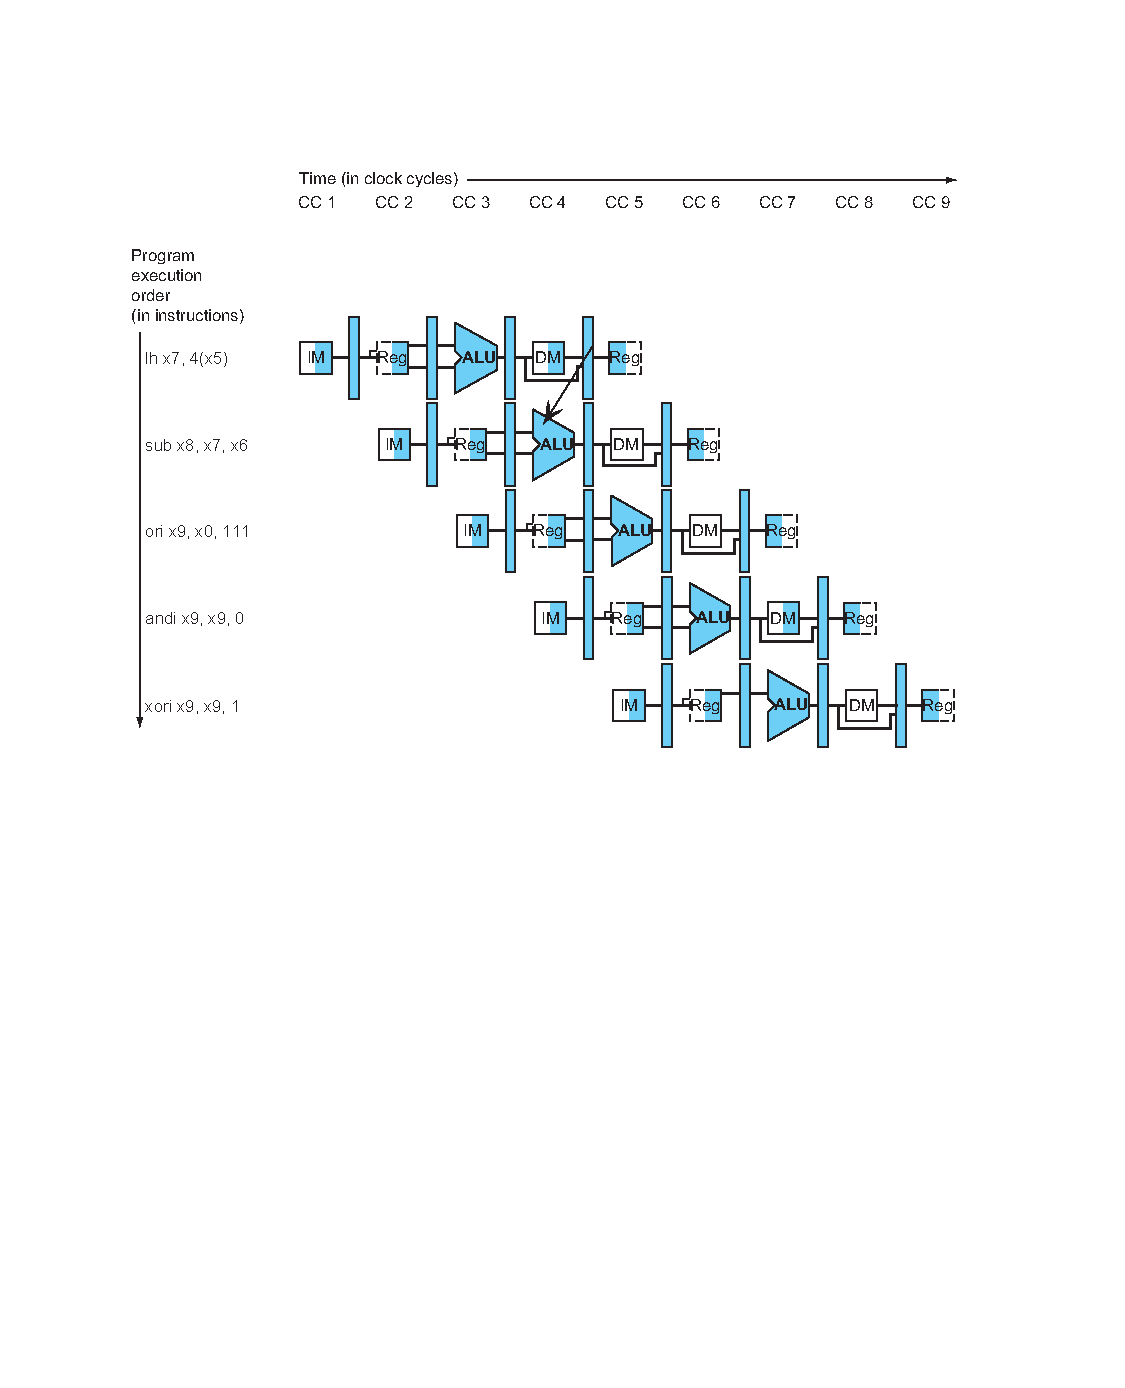
\includegraphics[scale=.9]{fig8.pdf}
	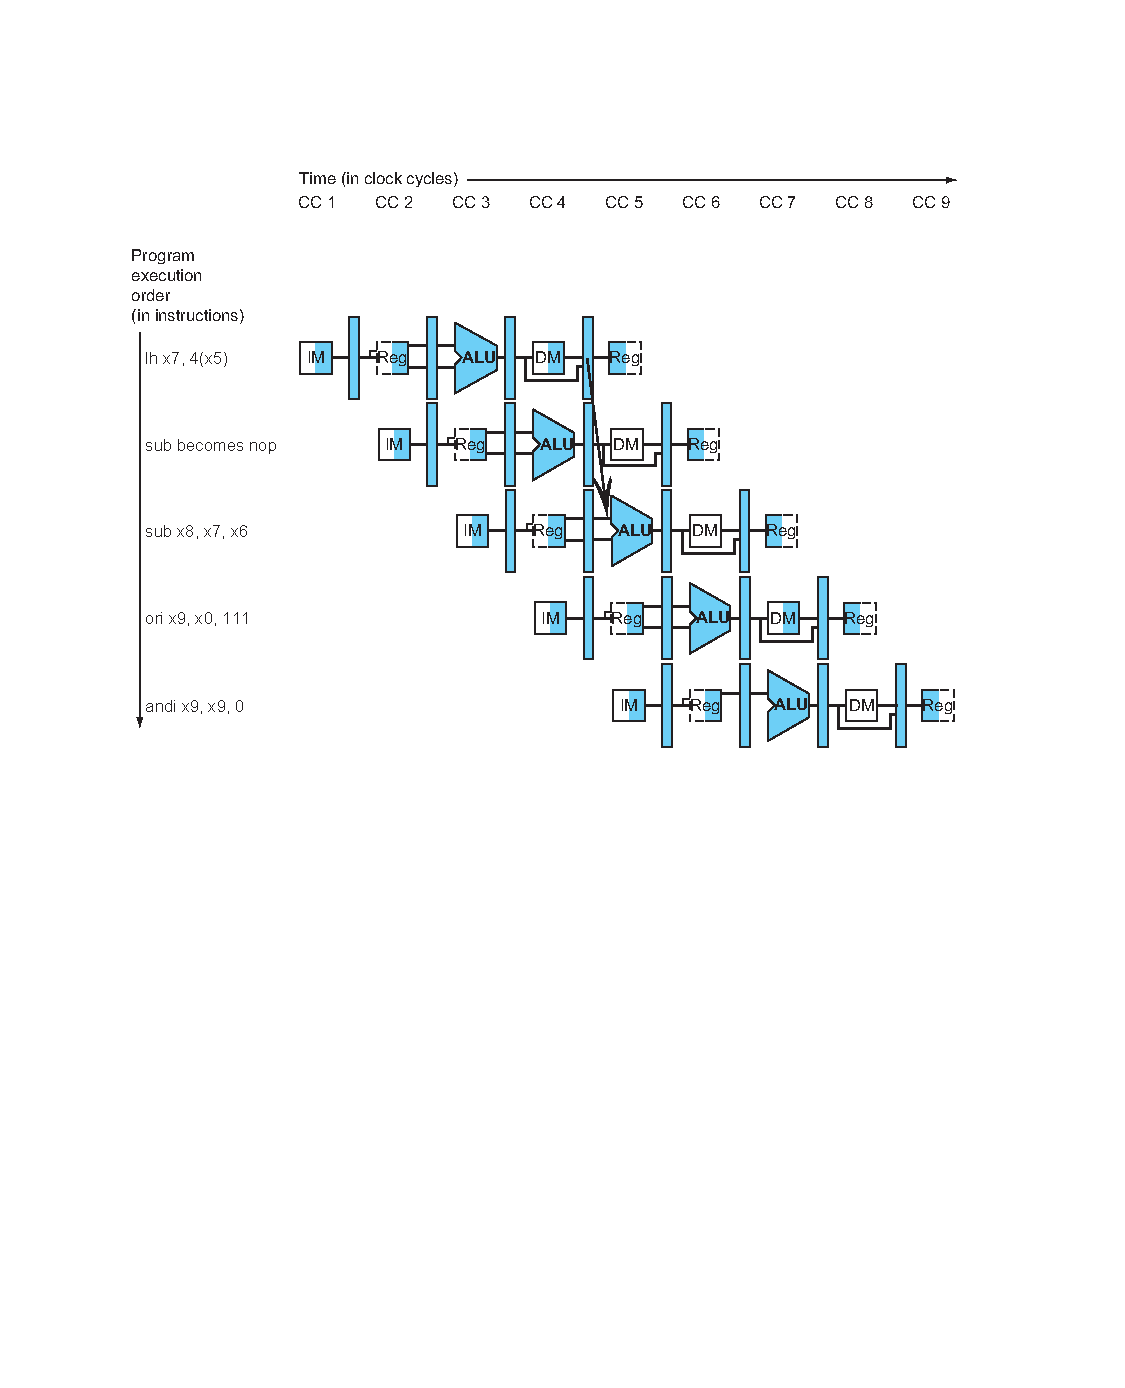
\includegraphics[scale=.9]{fig9.pdf}
	\caption{出现数据冒险和阻塞后的情况}
	\label{fig:label8}
\end{figure}

下一周期时,第6行代码仍在EX阶段,第5行代码执行WB阶段,此时MEM/WB里已有x7的值,通过旁路将其传入EX/MEM阶段即可。

如图\ref{fig:label10}、\ref{fig:label11}分别为第8周期、第9周期的仿真图像。

\begin{figure}
	\centering
	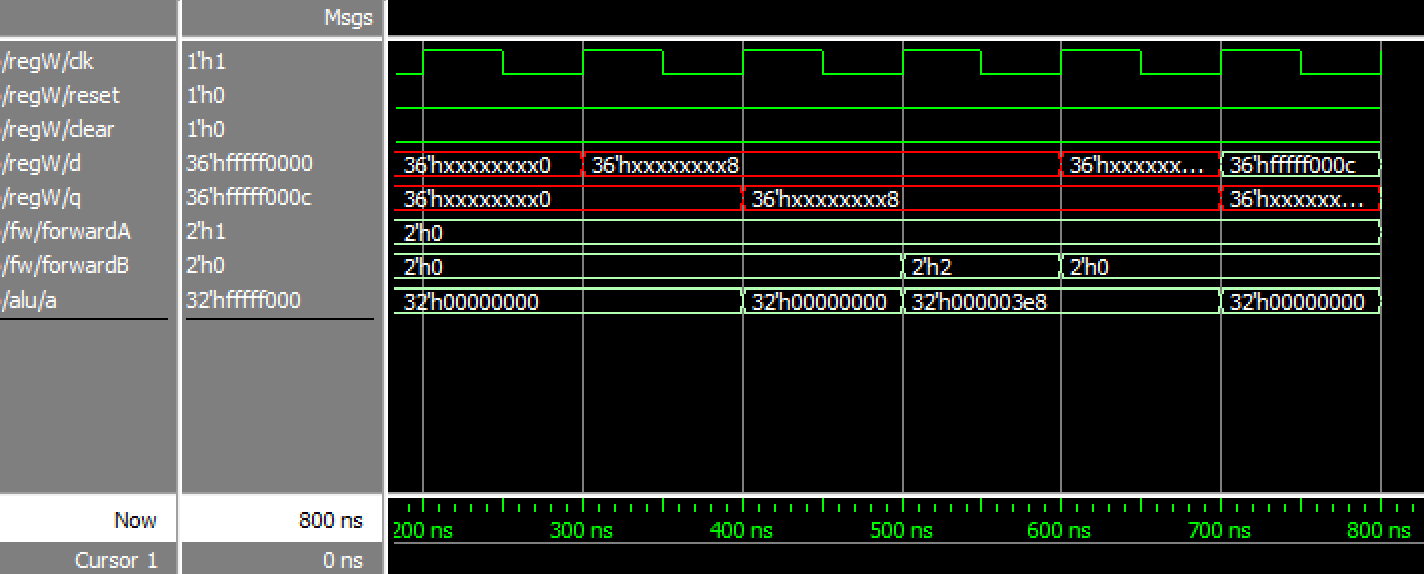
\includegraphics[scale=.8]{fig10.png}
	\caption{出现数据冒险时相关线路的仿真(第8周期)}
	\label{fig:label10}
\end{figure}

此时还没有x7的数据(0xffff0000)出现,所以无法将其前递到ALU的操作数$a$处。

\begin{figure}
	\centering
	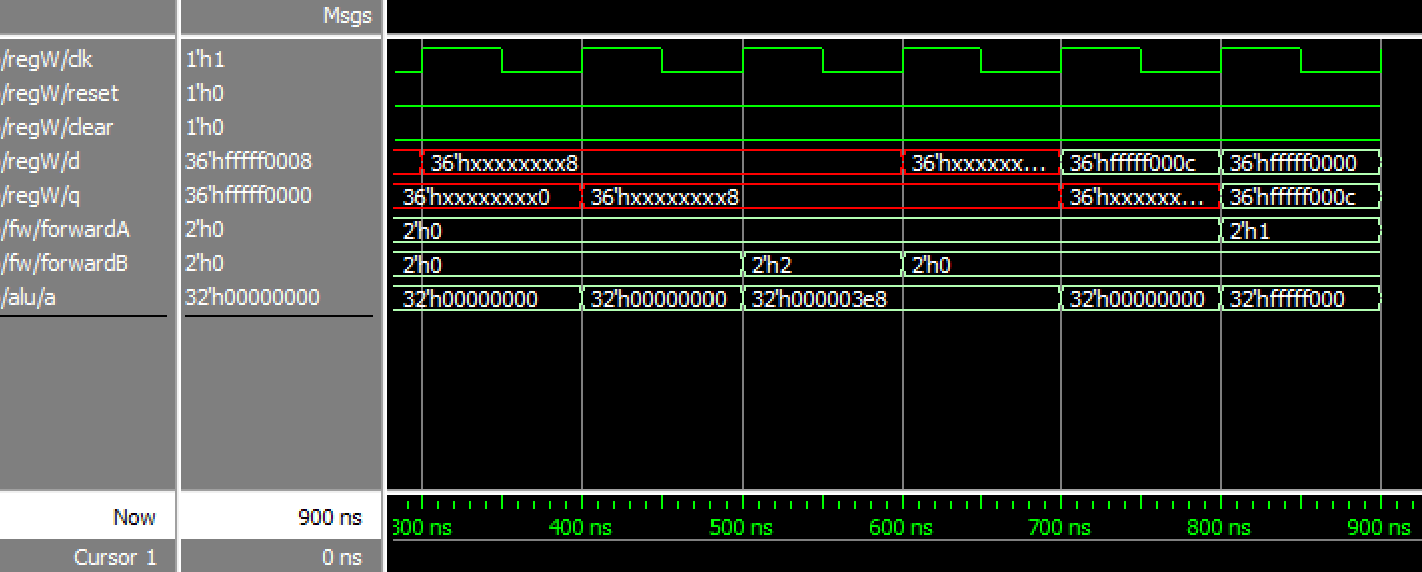
\includegraphics[scale=.8]{fig11.png}
	\caption{出现数据冒险后阻塞的仿真(第9周期)}
	\label{fig:label11}
\end{figure}

x7的数据(0xffff0000)出现在MEM/WB寄存器的输入,此时forwardA=01,即可将其前递到ALU的操作数$a$处。

\begin{figure}
	\centering
	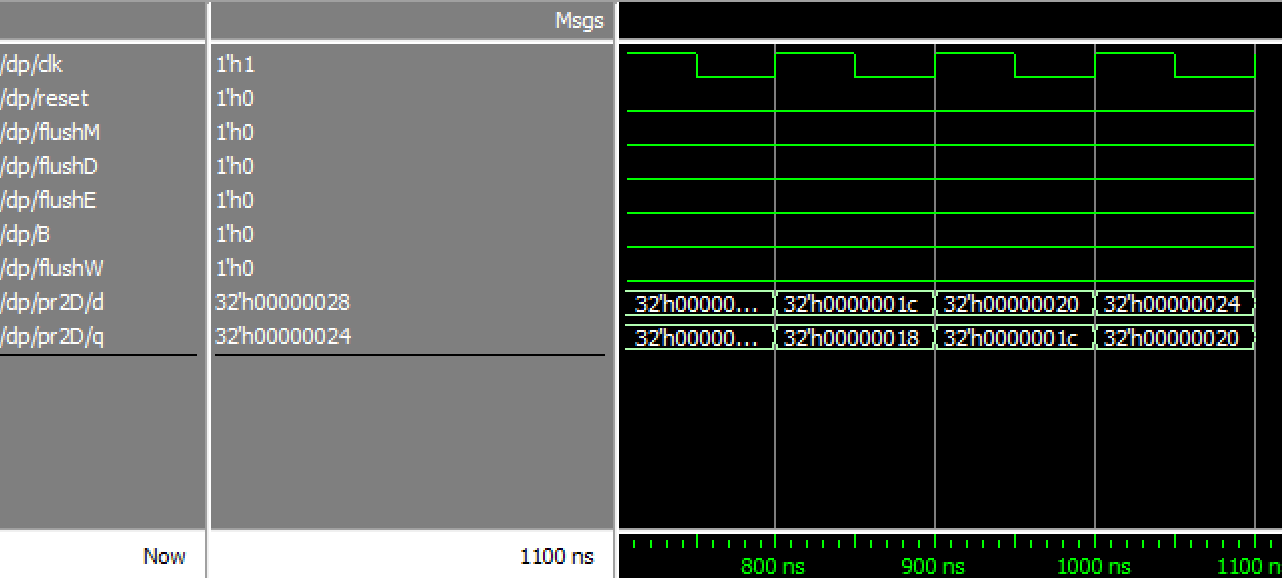
\includegraphics[scale=.8]{fig12.png}
	\caption{第12周期,跳转探测到之前}
	\label{fig:label12}
\end{figure}

\begin{figure}
	\centering
	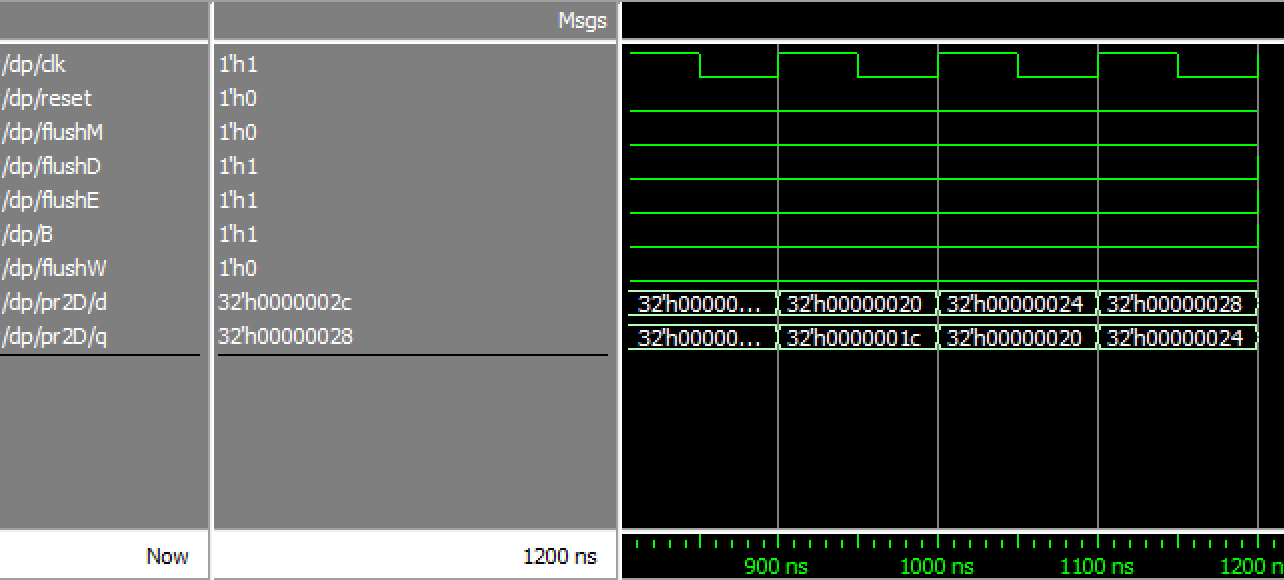
\includegraphics[scale=.8]{fig13.png}
	\caption{第13周期,探测到跳转}
	\label{fig:label13}
\end{figure}

\begin{figure}
	\centering
	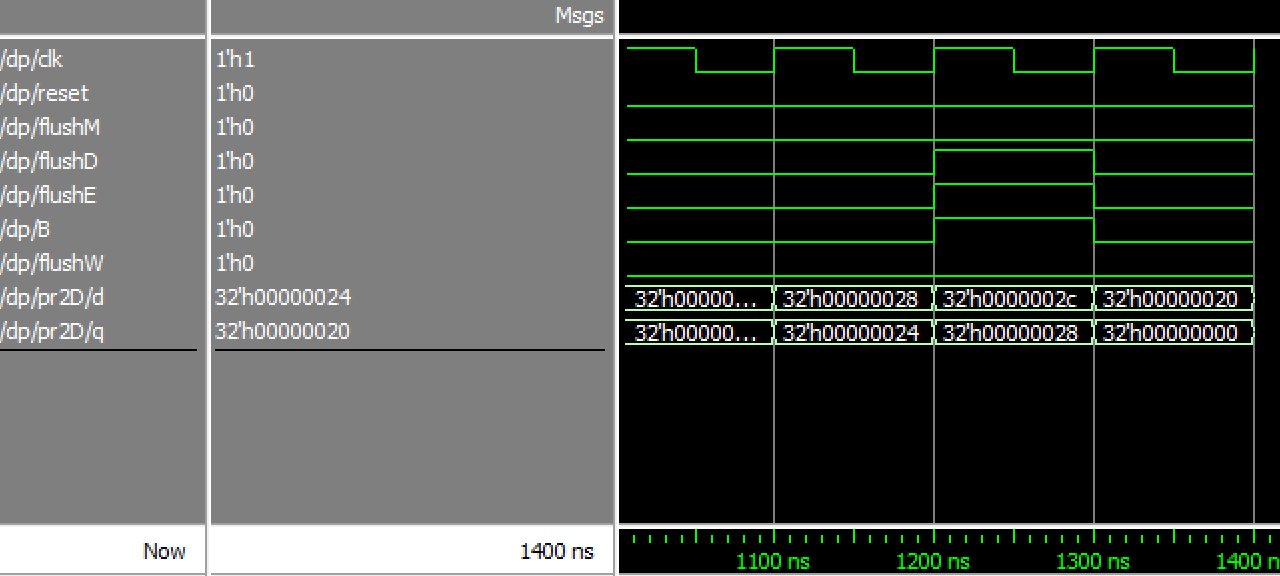
\includegraphics[scale=.8]{fig14.png}
	\caption{第14周期,跳转后PC=0x20}
	\label{fig:label14}
\end{figure}

\subsubsection{控制冒险}

执行到代码第11行时,出现了控制冒险。此时流水线中已经有12行及以后的代码,由于此时需要跳转,所以在流水线中EX阶段以前的部分需要被清除掉,重新读取新的PC地址的指令。

第12周期,指令{\tt bne x0, x9, skip1}仍在ID阶段,所有flush信号和B信号(探测到跳转发生)均为0。



第13周期,指令{\tt bne x0, x9, skip1}在EX阶段执行结束后,B信号跳变为1,同时flushD、flushE也跳变为1,此时这两层IF/ID,ID/EX寄存器即将被清空。清空后,流水线从PC=0x20的阶段继续执行。



\subsection{下载测试代码及分析}
	测试汇编代码在{\tt diy.asm}文件中。文件实现了 $6\times 8$ 的矩阵加载和游戏数据处理功能。
	
	在下载测试时,基于{\tt VGAIO.v}等文件,修改了TOP文件和总线文件使其支持VGA图像的扫描。为了方便起见,没有额外设置显存,而是在TOP文件里定义了48个寄存器,作为显示内容。
	
	根据上述技术基础,在本实验中设计了“方块消消乐”游戏。
	
	本实验结合拨码开关、按键输入、VGA输出、数码管输出四个交互式模块,设计了这款游戏。
	
	游戏简要规则为:将高亮光标移动至需要消灭的方块上,如果当前方块四周(四连通区域)有同样颜色的方块,按下消灭键即可将其全部消除。连通的数量越多,本次得分越多,得分在数码管上以16进制形式进行显示。
	
	当方块被消灭后,其上方的方块会由于重力掉落,因此游戏的玩法较为丰富,最终目的为达到尽可能高的分数。

\subsection{下载测试结果}

	如图所示,修改{\tt santi\_jitter.v}文件可以获取按键信号,从而操纵光标上下左右移动,并执行消灭操作。改变输入到七段数码管中的数据,可以实时显示当前得分。
	
	经测试,游戏主体部分结果正确,数码管可以正常显示,可以正常接收按键区信号,认为实验成功。
	
	汇编代码中有较多数据依赖和控制跳转,正常执行后说明流水线架构设计无误,可以正确处理数据冒险等可能存在的问题。
	
\begin{figure}
	\centering
	\subfloat[游戏初始画面]{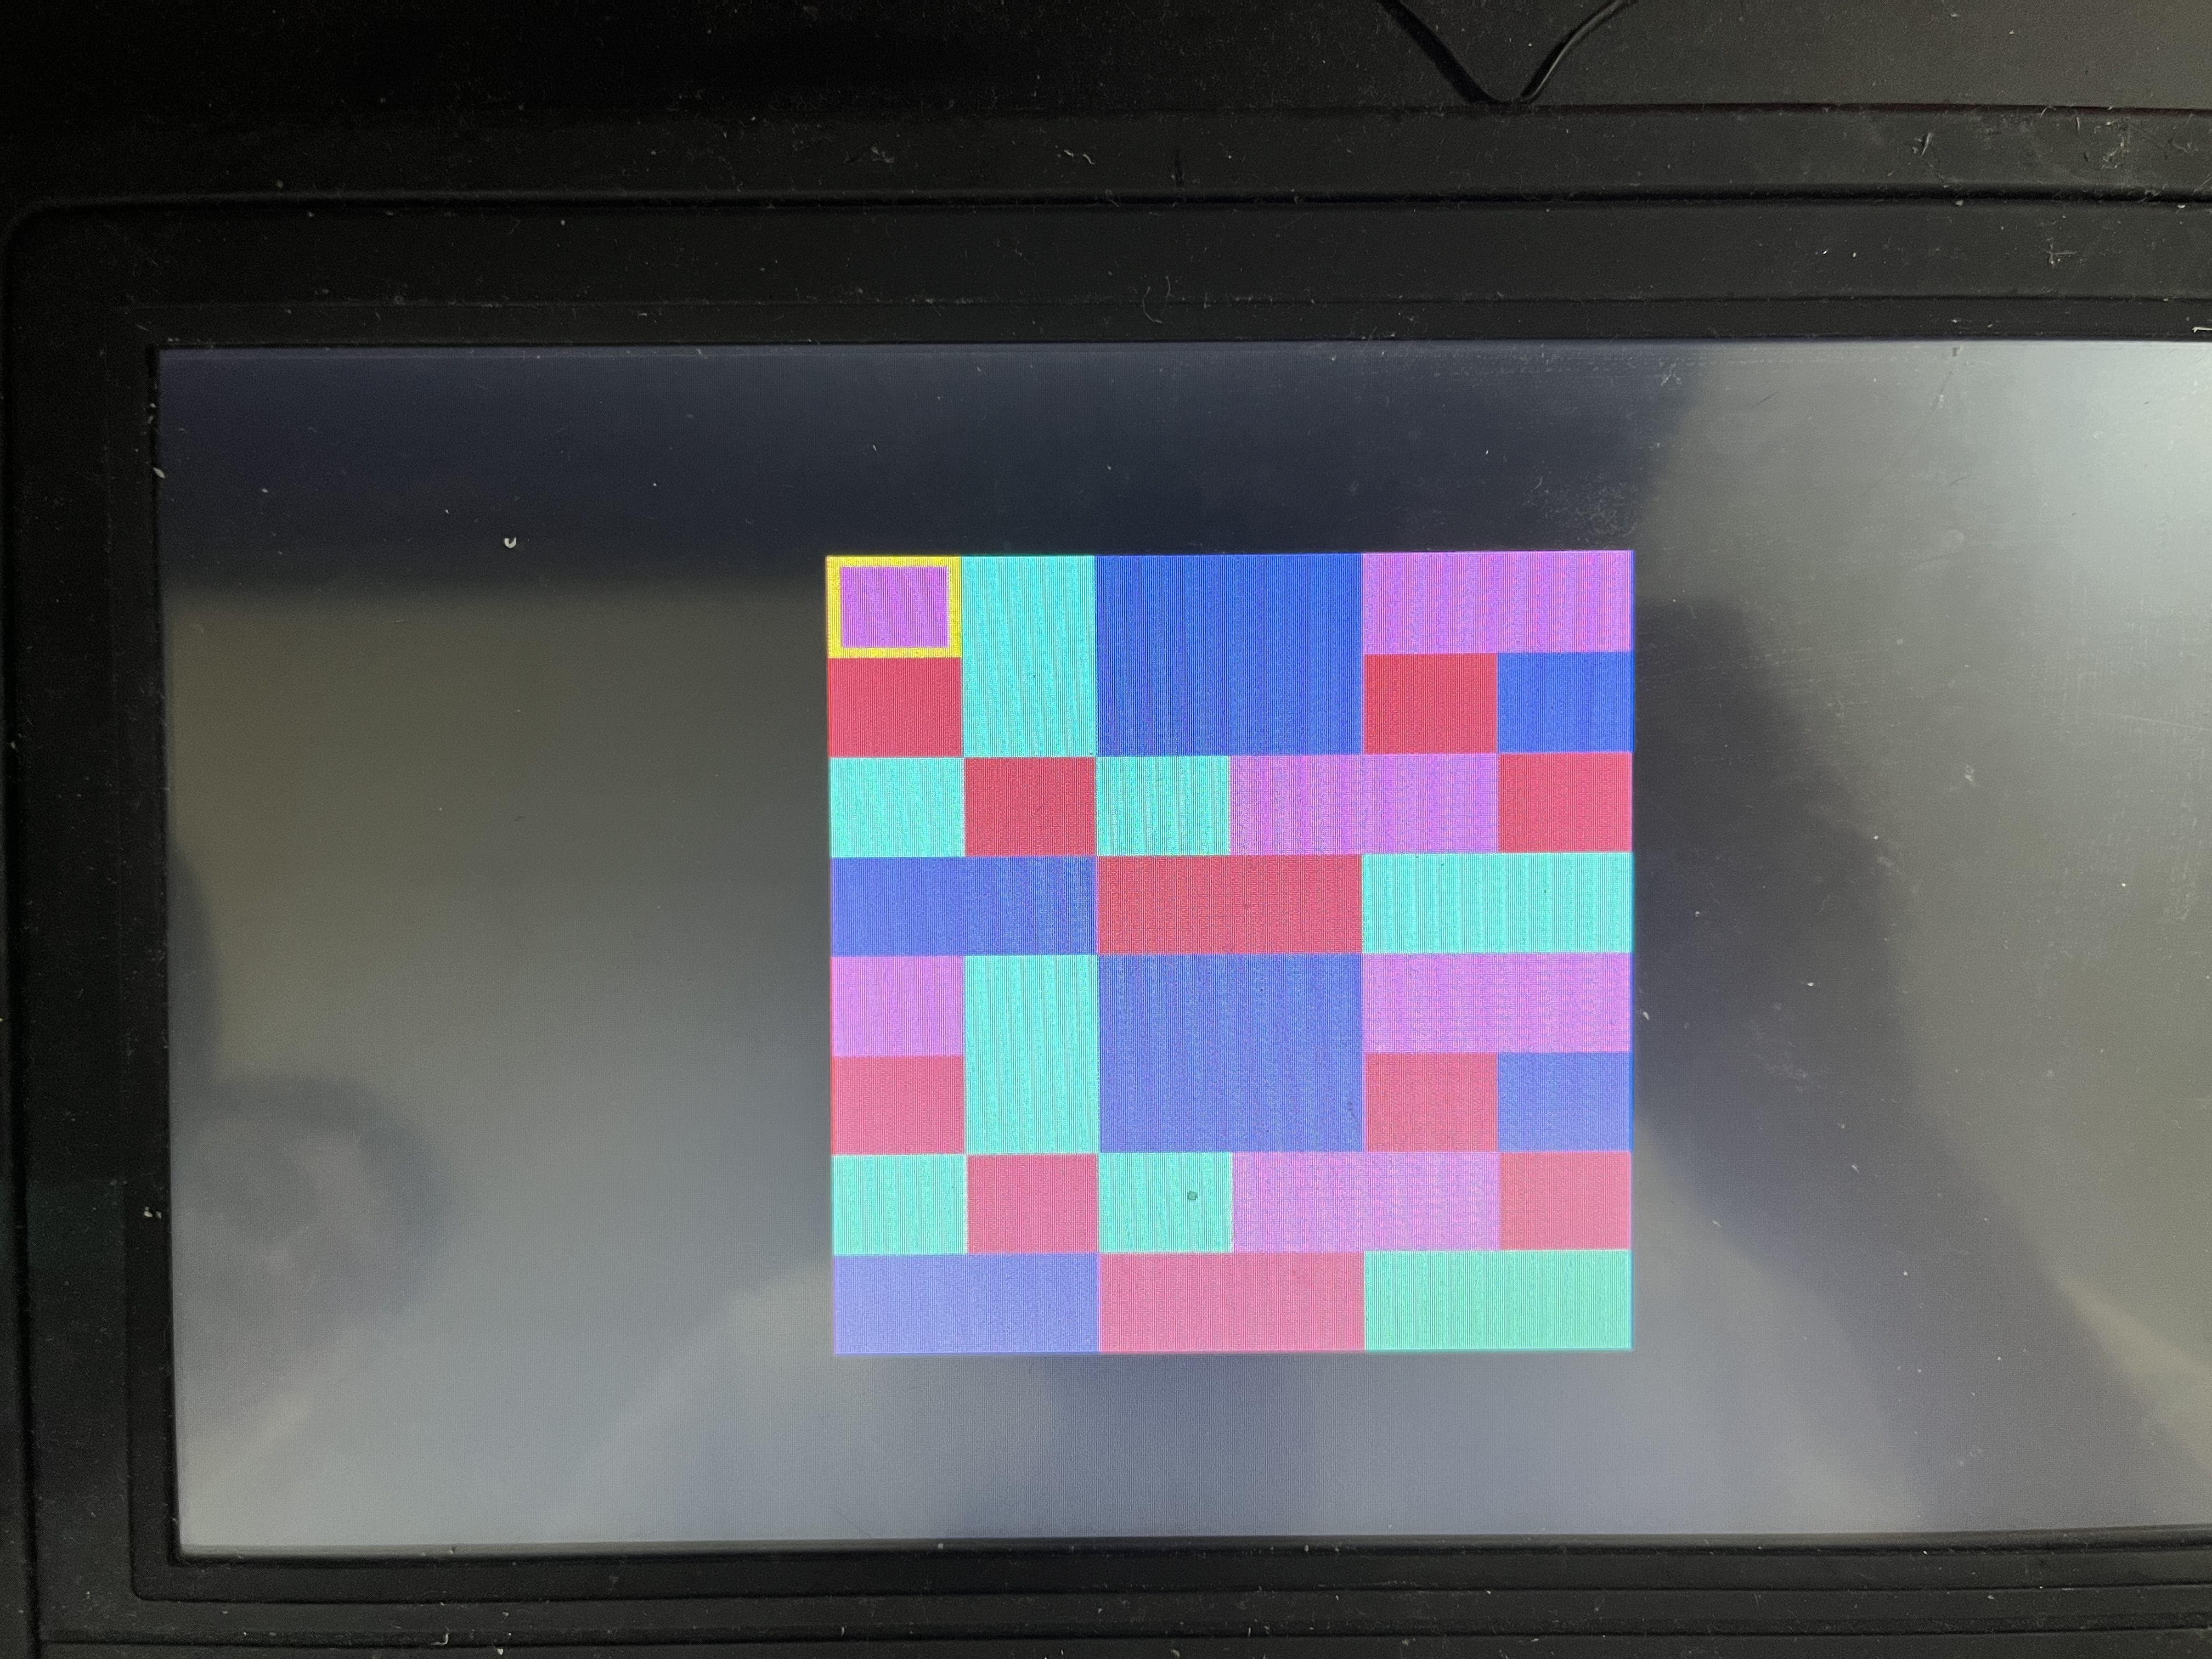
\includegraphics[width=.4\linewidth]{sf1.jpg}}\hspace{5pt}
	\subfloat[按键交互部分]{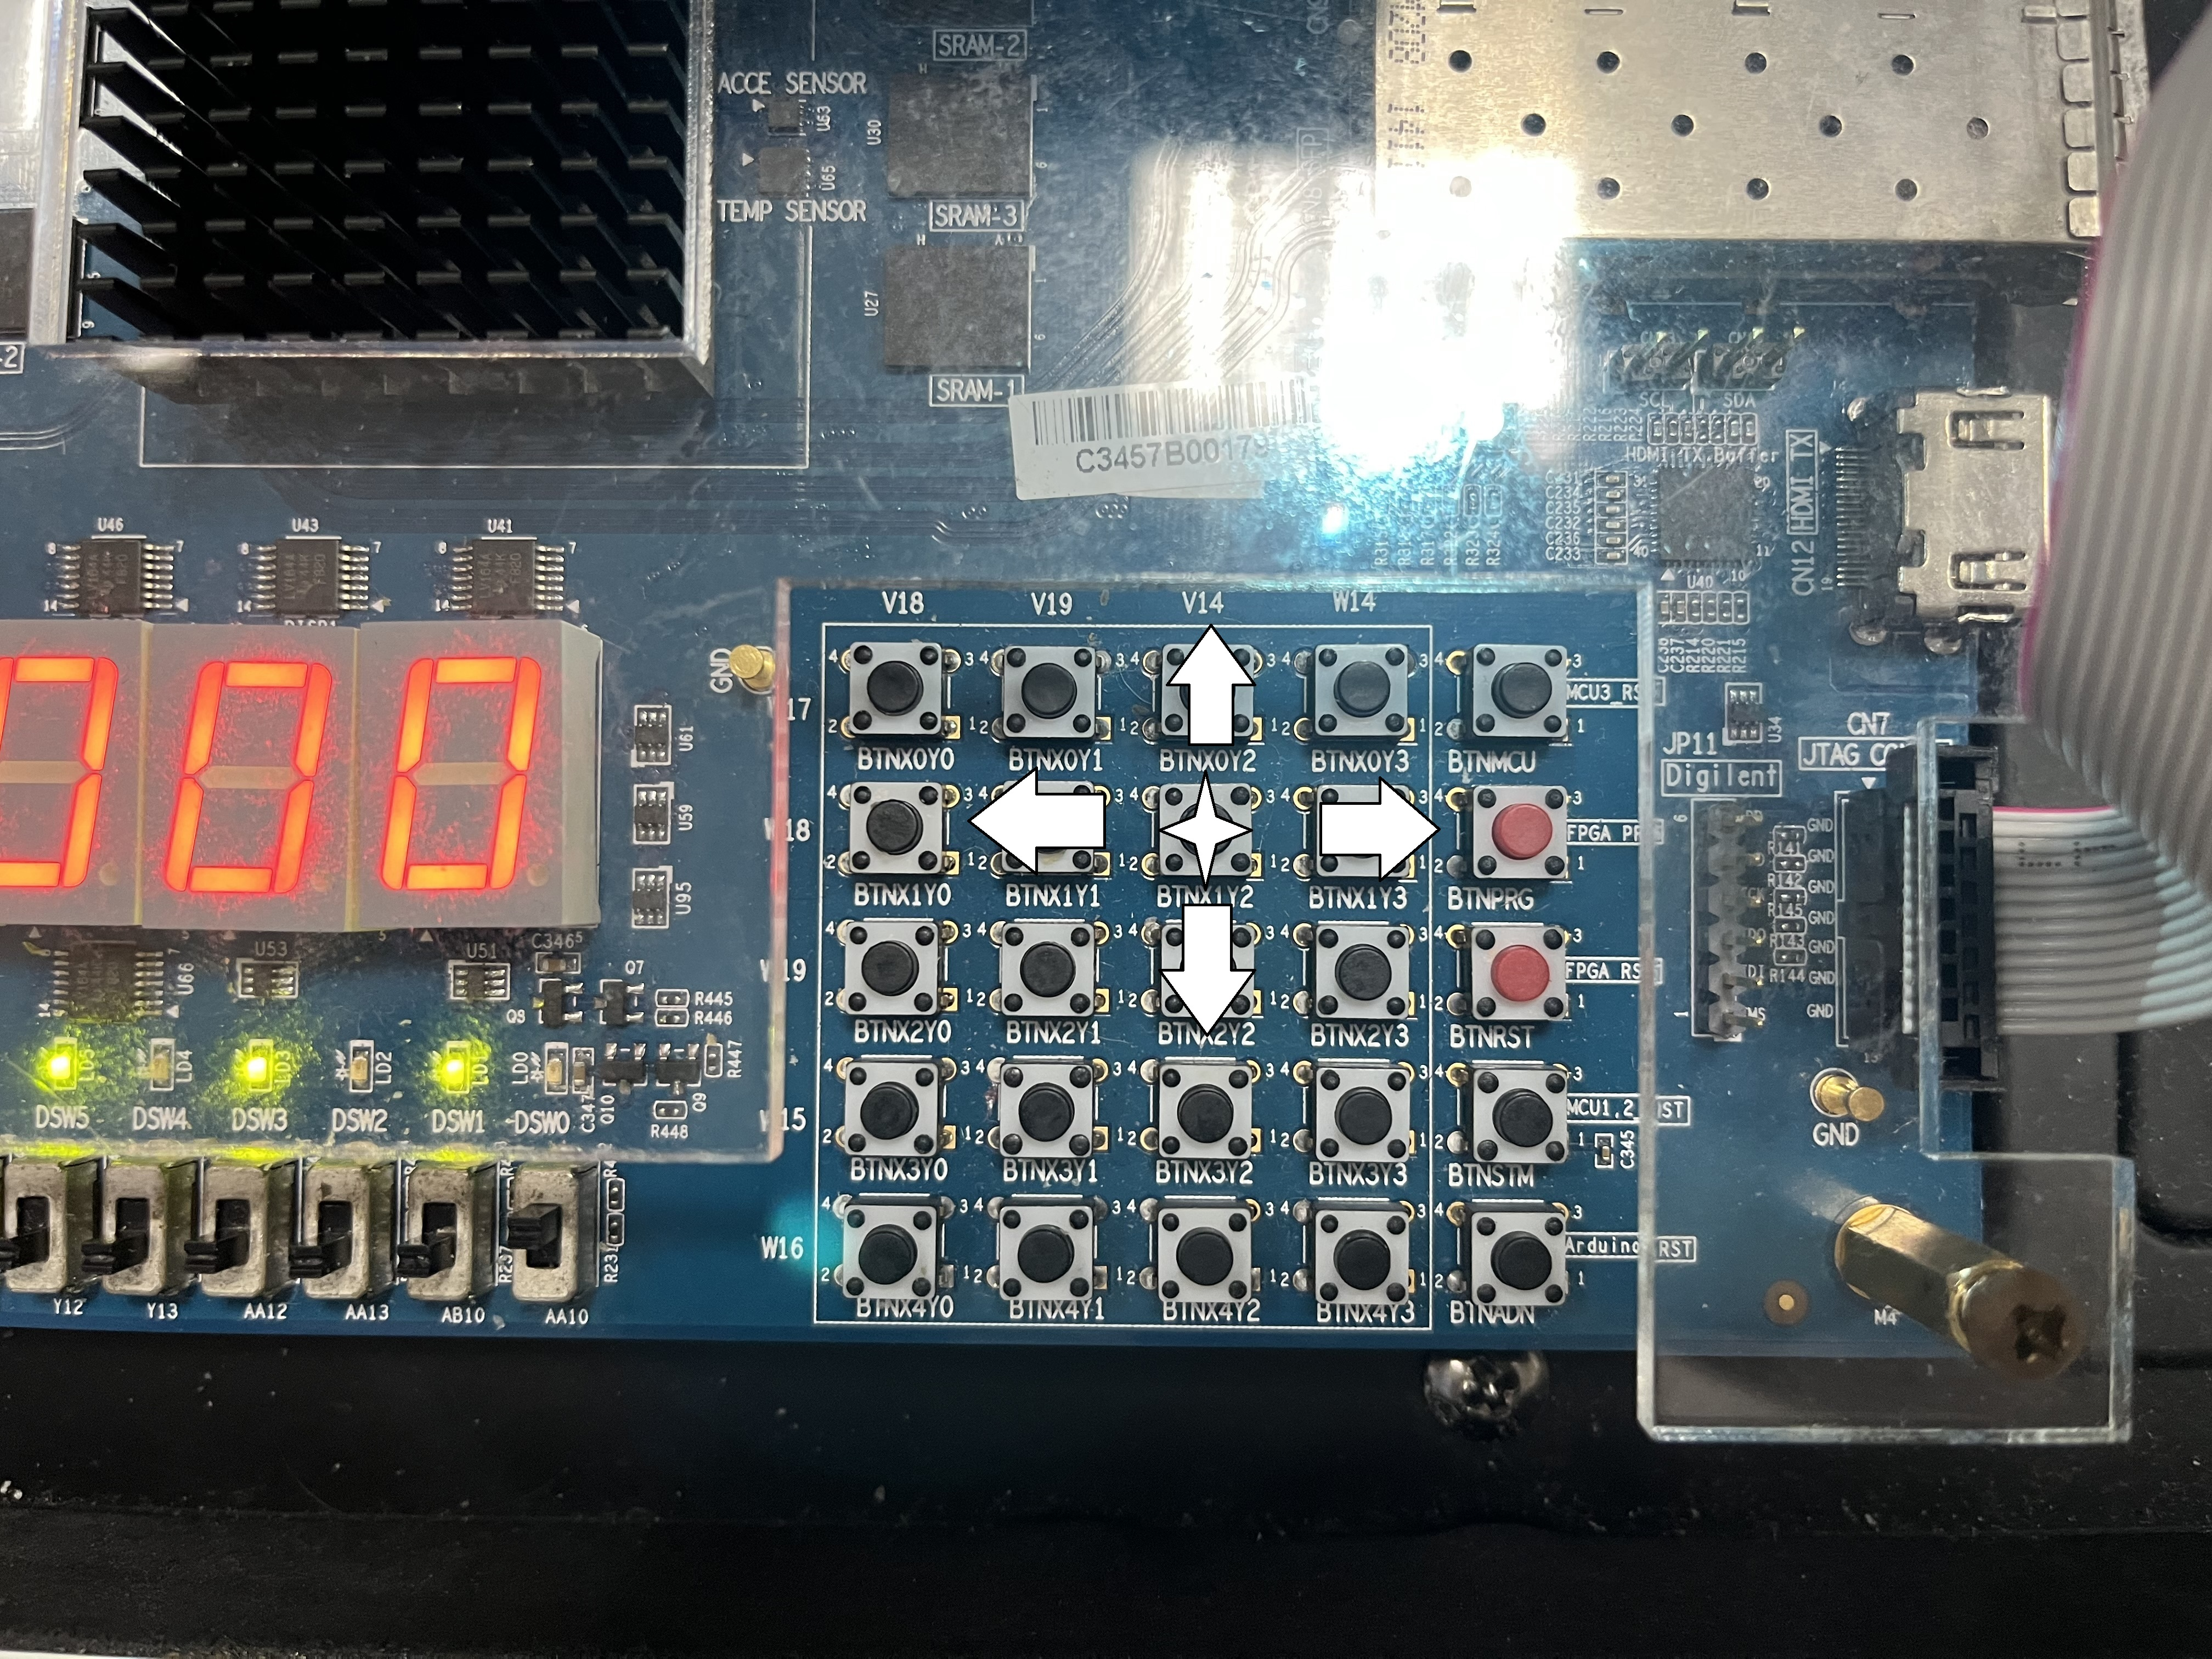
\includegraphics[width=.4\linewidth]{sf2.jpg}}\vspace{1pt}
	\subfloat[游戏过程中]{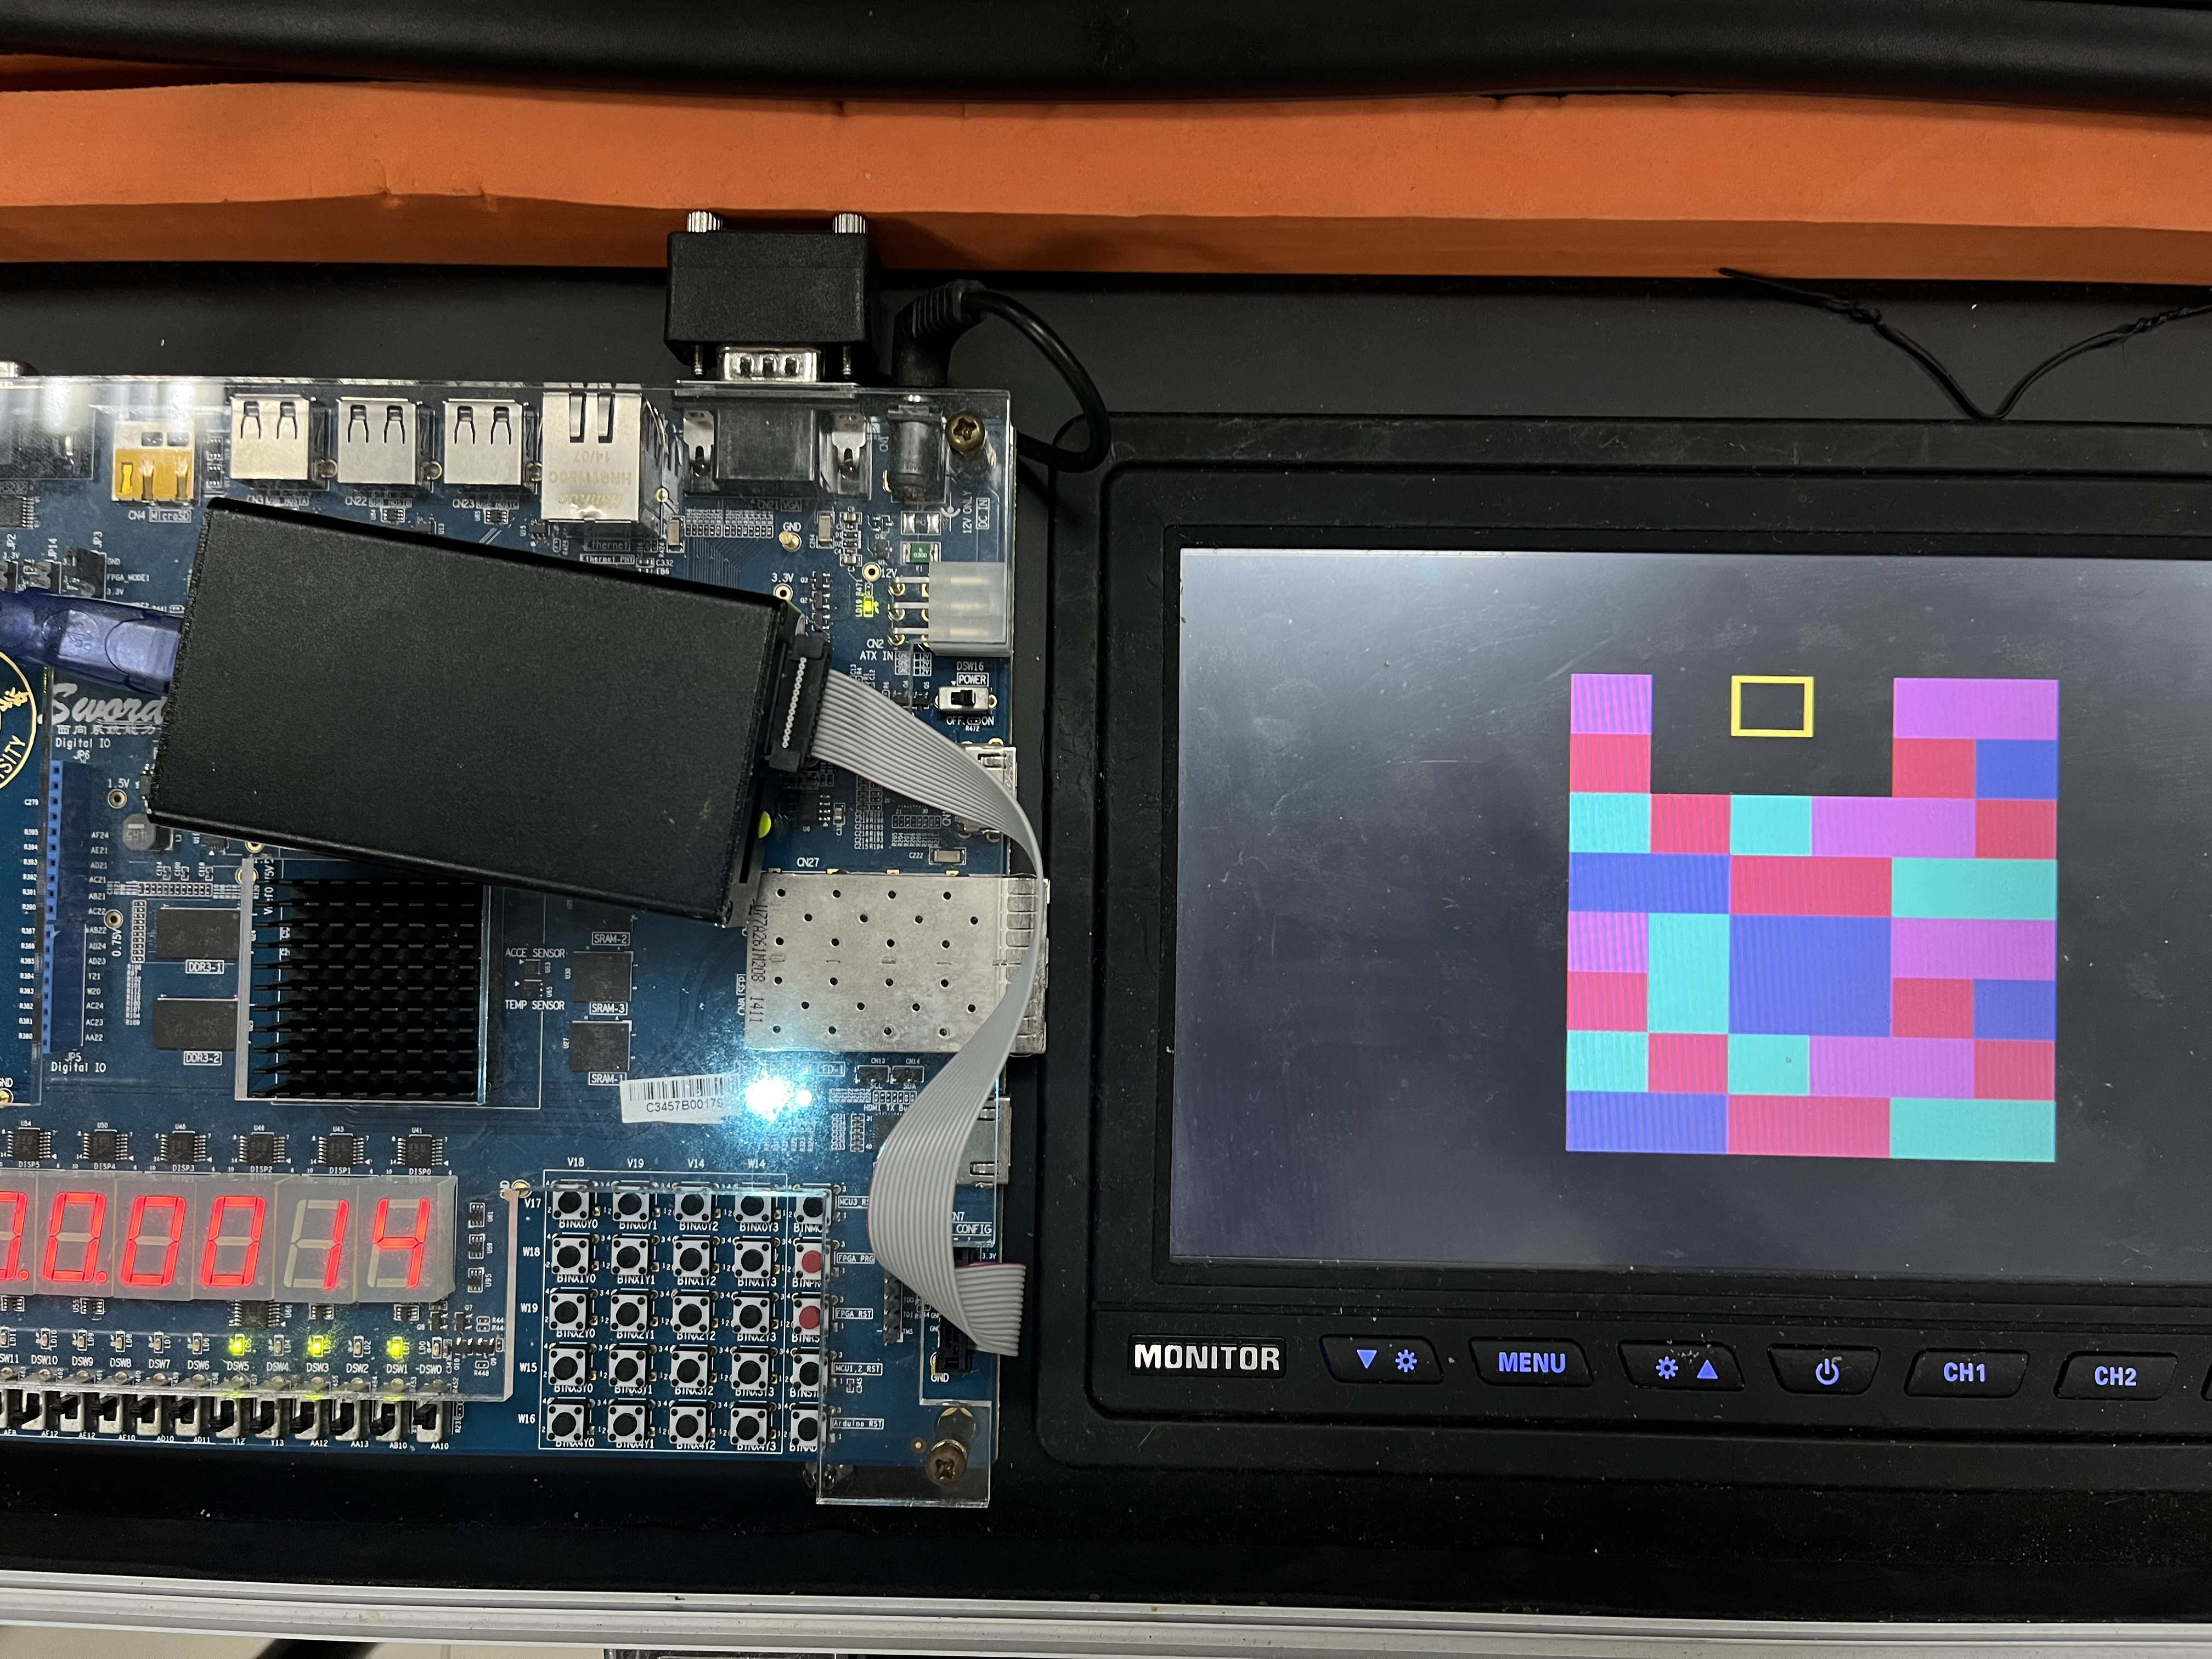
\includegraphics[width=.4\linewidth]{sf3.jpg}}\hspace{5pt}
	\subfloat[游戏结果]{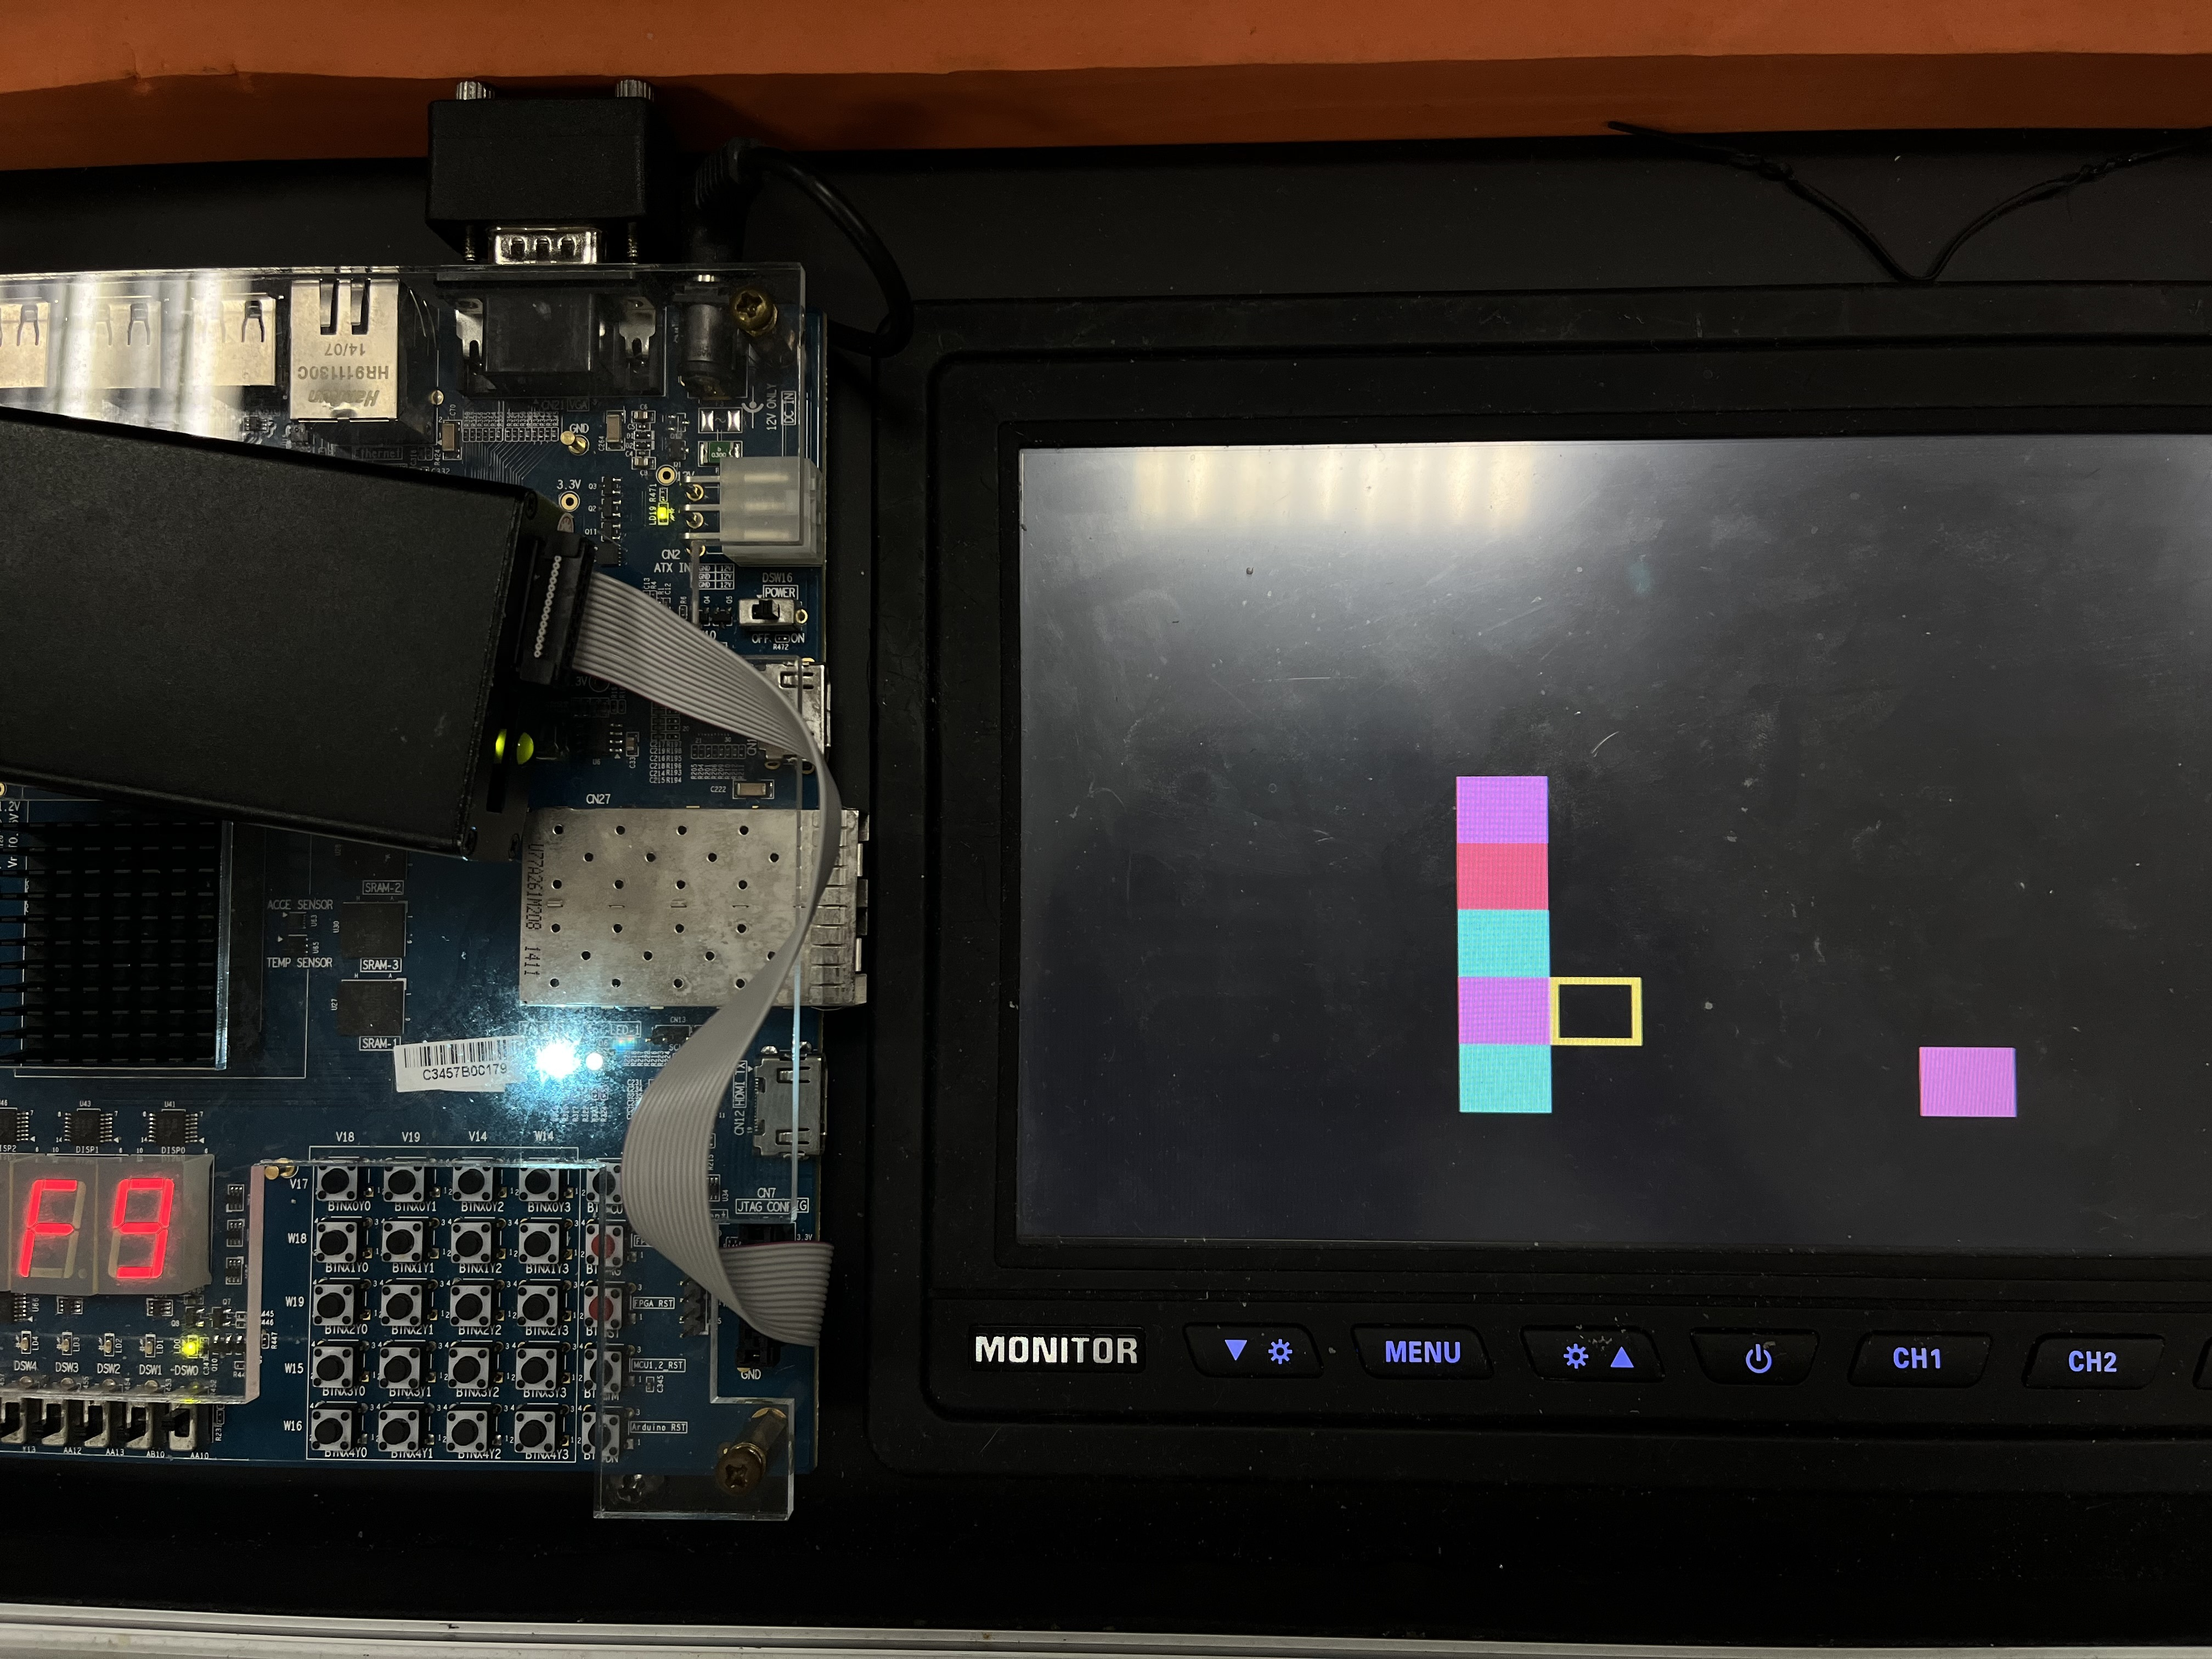
\includegraphics[width=.4\linewidth]{sf4.jpg}}
	\caption{基于本实验设计的“方块消消乐”游戏}
\end{figure}

\section{实验总结}
\subsection{实验总结}
	本实验是基于RISC-V架构设计的单周期、流水线CPU,同时根据SWORD开发板特性设计了额外的交互式内容。实验具有较大的挑战性,一方面使用了Verilog这一不同于其他高级语言的设计方式,另一方面在复杂的数据周转和信号变化中,调试是一件非常困难的事情。
	
	实现一个CPU并不难,但要将单周期CPU改进为流水线并支持数据冒险,就是非常考验能力的任务。数据并不只是单向流动,上升沿和下降沿、阻塞和非阻塞的判断都会对数字电路的实现造成非常大的影响,因此能够完整做出本实验,也是对能力的认可和自我的挑战。
	
	在交互式内容中,VGA、按钮等相对陌生的环境往往需要数十小时甚至几天的时间来摸索和实验,在这期间和老师同学的互相交流和上网查阅资料的能力也显得尤为重要,但最主要的还是动手实践能力。
	
	不过,在按钮实现时,也遇到了较多软硬件结合(Verilog和汇编结合)才能解决的情况。游戏的最终版本仍存在按钮响应的问题,在今后的设计实验中仍需加强设计的健壮性。
	
	最终,VGA显示正确,代码正常执行,寄存器和内存内容和Venus平台一致,说明实验成功。
\subsection{取得的收获}
	在这段实验的过程中,我提升了自己的学习能力、动手实践能力、解决创新型问题的能力;也将汇编语言程序设计和Verilog编程的能力进行了巩固。
	
	在进行流水线CPU课间实验时,我受到提交方式的启发,经常将自己的代码上传github仓库进行备份,一方面防止丢失,另一方面方便多设备同步,最重要的一点是方便回退版本。在设计实验过程中不仅仅培养的是专业能力,也有应用扩展和解决问题的能力。
	
	在完成流水线CPU的过程中,我遇到了时序判断和逻辑信号的多重困难,尤其是莫名其妙出现的X信号,我对此深感困惑。后来我发现ModelSim软件可以单步调试,并实时观察每个信号的数据情况,在这之后我解决问题的速度有了显著的提升。而对于X信号产生的原因,主要是输入信号存在未定义的可能性。
	
	此外,在实验过程中遇到的其他问题,也引发了我的思考,如果出现了难以解决的问题,就刨根问底找到问题的根源,将提供的原始元件的原理研究清楚,最终解决问题或更换元件。
	
	本实验培养了我的探究性精神,也让我在完成这项“大工程”后有着自豪的成就感和满足感。计算机不是只有软件,也不是只有硬件,只有在软硬件和学科交叉相结合之下,计算机的最大作用才能发挥出来,这也是它的魅力所在。
\newpage
\begin{thebibliography}{99}  
	
	\bibitem{ref1}David A. P, John L.H, 计算机组成与设计:硬件/软件接口[M].易江芳,刘先华.北京:机械工业出版社,2020.
	\bibitem{ref2}芮雪,王亮亮,杨琴.国产处理器研究与发展现状综述[J].现代计算机(专业版),2014(08):15-19.
	\bibitem{ref3}潘树朋,刘有耀.RISC-V微处理器以及商业IP的综述[J].单片机与嵌入式系统应用,2020,20(06):5-8+12.
	\bibitem{ref4}全球首颗智能穿戴领域人工智能芯片发布[J].智能城市,2019,5(10):191.
	\bibitem{ref5}雷思磊.RISC-V架构的开源处理器及SoC研究综述[J].单片机与嵌入式系统应用,2017,17(02):56-60+76.
	\bibitem{ref6}袁攀. 基于嵌入式RISC-V微处理器的流水线研究与设计[D].长沙理工大学,2021.DOI:10.26985/d.cnki.gcsjc.2021.000811.
	\bibitem{ref7}李亚民.计算机原理与设计:Verilog HDL版[M].北京:清华大学出版社,2011.
	
\end{thebibliography}
\newpage
\begin{center}
	\zihao{3} 教师评语评分
\end{center}

\zihao{4} \noindent 评语:\underline{\hspace{14.5cm}}

\vspace{10pt}
\underline{\hspace{15cm}}

\vspace{10pt}
\underline{\hspace{15cm}}

\vspace{10pt}
\underline{\hspace{15cm}}

\vspace{10pt}
\underline{\hspace{15cm}}

\vspace{10pt}
\underline{\hspace{15cm}}

\vspace{10pt}
\underline{\hspace{15cm}}

\vspace{10pt}
\underline{\hspace{15cm}}

\vspace{10pt}

\hspace{6cm}评阅人:\underline{\hspace{5cm}}

\hspace{9cm}年\quad\qquad 月\quad\qquad 日

\noindent\nolinebreak(备注:对该实验报告给予优点和不足的评价,并给出百分制评分。)

\end{document}